% Options for packages loaded elsewhere
\PassOptionsToPackage{unicode}{hyperref}
\PassOptionsToPackage{hyphens}{url}
\PassOptionsToPackage{dvipsnames,svgnames,x11names}{xcolor}
%
\documentclass[
  man,floatsintext]{apa7}
\usepackage{amsmath,amssymb}
\usepackage{iftex}
\ifPDFTeX
  \usepackage[T1]{fontenc}
  \usepackage[utf8]{inputenc}
  \usepackage{textcomp} % provide euro and other symbols
\else % if luatex or xetex
  \usepackage{unicode-math} % this also loads fontspec
  \defaultfontfeatures{Scale=MatchLowercase}
  \defaultfontfeatures[\rmfamily]{Ligatures=TeX,Scale=1}
\fi
\usepackage{lmodern}
\ifPDFTeX\else
  % xetex/luatex font selection
\fi
% Use upquote if available, for straight quotes in verbatim environments
\IfFileExists{upquote.sty}{\usepackage{upquote}}{}
\IfFileExists{microtype.sty}{% use microtype if available
  \usepackage[]{microtype}
  \UseMicrotypeSet[protrusion]{basicmath} % disable protrusion for tt fonts
}{}
\makeatletter
\@ifundefined{KOMAClassName}{% if non-KOMA class
  \IfFileExists{parskip.sty}{%
    \usepackage{parskip}
  }{% else
    \setlength{\parindent}{0pt}
    \setlength{\parskip}{6pt plus 2pt minus 1pt}}
}{% if KOMA class
  \KOMAoptions{parskip=half}}
\makeatother
\usepackage{xcolor}
\usepackage{graphicx}
\makeatletter
\def\maxwidth{\ifdim\Gin@nat@width>\linewidth\linewidth\else\Gin@nat@width\fi}
\def\maxheight{\ifdim\Gin@nat@height>\textheight\textheight\else\Gin@nat@height\fi}
\makeatother
% Scale images if necessary, so that they will not overflow the page
% margins by default, and it is still possible to overwrite the defaults
% using explicit options in \includegraphics[width, height, ...]{}
\setkeys{Gin}{width=\maxwidth,height=\maxheight,keepaspectratio}
% Set default figure placement to htbp
\makeatletter
\def\fps@figure{htbp}
\makeatother
\setlength{\emergencystretch}{3em} % prevent overfull lines
\providecommand{\tightlist}{%
  \setlength{\itemsep}{0pt}\setlength{\parskip}{0pt}}
\setcounter{secnumdepth}{-\maxdimen} % remove section numbering
% Make \paragraph and \subparagraph free-standing
\ifx\paragraph\undefined\else
  \let\oldparagraph\paragraph
  \renewcommand{\paragraph}[1]{\oldparagraph{#1}\mbox{}}
\fi
\ifx\subparagraph\undefined\else
  \let\oldsubparagraph\subparagraph
  \renewcommand{\subparagraph}[1]{\oldsubparagraph{#1}\mbox{}}
\fi
% definitions for citeproc citations
\NewDocumentCommand\citeproctext{}{}
\NewDocumentCommand\citeproc{mm}{%
  \begingroup\def\citeproctext{#2}\cite{#1}\endgroup}
\makeatletter
 % allow citations to break across lines
 \let\@cite@ofmt\@firstofone
 % avoid brackets around text for \cite:
 \def\@biblabel#1{}
 \def\@cite#1#2{{#1\if@tempswa , #2\fi}}
\makeatother
\newlength{\cslhangindent}
\setlength{\cslhangindent}{1.5em}
\newlength{\csllabelwidth}
\setlength{\csllabelwidth}{3em}
\newenvironment{CSLReferences}[2] % #1 hanging-indent, #2 entry-spacing
 {\begin{list}{}{%
  \setlength{\itemindent}{0pt}
  \setlength{\leftmargin}{0pt}
  \setlength{\parsep}{0pt}
  % turn on hanging indent if param 1 is 1
  \ifodd #1
   \setlength{\leftmargin}{\cslhangindent}
   \setlength{\itemindent}{-1\cslhangindent}
  \fi
  % set entry spacing
  \setlength{\itemsep}{#2\baselineskip}}}
 {\end{list}}
\usepackage{calc}
\newcommand{\CSLBlock}[1]{\hfill\break\parbox[t]{\linewidth}{\strut\ignorespaces#1\strut}}
\newcommand{\CSLLeftMargin}[1]{\parbox[t]{\csllabelwidth}{\strut#1\strut}}
\newcommand{\CSLRightInline}[1]{\parbox[t]{\linewidth - \csllabelwidth}{\strut#1\strut}}
\newcommand{\CSLIndent}[1]{\hspace{\cslhangindent}#1}
\ifLuaTeX
\usepackage[bidi=basic]{babel}
\else
\usepackage[bidi=default]{babel}
\fi
\babelprovide[main,import]{english}
% get rid of language-specific shorthands (see #6817):
\let\LanguageShortHands\languageshorthands
\def\languageshorthands#1{}
% Manuscript styling
\usepackage{upgreek}
\captionsetup{font=singlespacing,justification=justified}

% Table formatting
\usepackage{longtable}
\usepackage{lscape}
% \usepackage[counterclockwise]{rotating}   % Landscape page setup for large tables
\usepackage{multirow}		% Table styling
\usepackage{tabularx}		% Control Column width
\usepackage[flushleft]{threeparttable}	% Allows for three part tables with a specified notes section
\usepackage{threeparttablex}            % Lets threeparttable work with longtable

% Create new environments so endfloat can handle them
% \newenvironment{ltable}
%   {\begin{landscape}\centering\begin{threeparttable}}
%   {\end{threeparttable}\end{landscape}}
\newenvironment{lltable}{\begin{landscape}\centering\begin{ThreePartTable}}{\end{ThreePartTable}\end{landscape}}

% Enables adjusting longtable caption width to table width
% Solution found at http://golatex.de/longtable-mit-caption-so-breit-wie-die-tabelle-t15767.html
\makeatletter
\newcommand\LastLTentrywidth{1em}
\newlength\longtablewidth
\setlength{\longtablewidth}{1in}
\newcommand{\getlongtablewidth}{\begingroup \ifcsname LT@\roman{LT@tables}\endcsname \global\longtablewidth=0pt \renewcommand{\LT@entry}[2]{\global\advance\longtablewidth by ##2\relax\gdef\LastLTentrywidth{##2}}\@nameuse{LT@\roman{LT@tables}} \fi \endgroup}

% \setlength{\parindent}{0.5in}
% \setlength{\parskip}{0pt plus 0pt minus 0pt}

% Overwrite redefinition of paragraph and subparagraph by the default LaTeX template
% See https://github.com/crsh/papaja/issues/292
\makeatletter
\renewcommand{\paragraph}{\@startsection{paragraph}{4}{\parindent}%
  {0\baselineskip \@plus 0.2ex \@minus 0.2ex}%
  {-1em}%
  {\normalfont\normalsize\bfseries\itshape\typesectitle}}

\renewcommand{\subparagraph}[1]{\@startsection{subparagraph}{5}{1em}%
  {0\baselineskip \@plus 0.2ex \@minus 0.2ex}%
  {-\z@\relax}%
  {\normalfont\normalsize\itshape\hspace{\parindent}{#1}\textit{\addperi}}{\relax}}
\makeatother

\makeatletter
\usepackage{etoolbox}
\patchcmd{\maketitle}
  {\section{\normalfont\normalsize\abstractname}}
  {\section*{\normalfont\normalsize\abstractname}}
  {}{\typeout{Failed to patch abstract.}}
\patchcmd{\maketitle}
  {\section{\protect\normalfont{\@title}}}
  {\section*{\protect\normalfont{\@title}}}
  {}{\typeout{Failed to patch title.}}
\makeatother

\usepackage{xpatch}
\makeatletter
\xapptocmd\appendix
  {\xapptocmd\section
    {\addcontentsline{toc}{section}{\appendixname\ifoneappendix\else~\theappendix\fi\\: #1}}
    {}{\InnerPatchFailed}%
  }
{}{\PatchFailed}
\usepackage{csquotes}
\usepackage[document]{ragged2e}
\usepackage{upgreek}
\usepackage{hyperref}
\usepackage{url}      % for \url command
\usepackage{caption}
\usepackage{orcidlink}
\usepackage{colortbl}
\usepackage{upquote}
\usepackage{textcomp}
\usepackage[document]{ragged2e}
\usepackage{dcolumn}
\usepackage{setspace}
\AtBeginEnvironment{tabular}{\doublespacing}
\AtBeginEnvironment{lltable}{\doublespacing}
\AtBeginEnvironment{tablenotes}{\singlespacing}
\captionsetup[table]{font={stretch=1}}
\captionsetup[figure]{font={stretch=1}}
\raggedbottom
\pagenumbering{gobble}
\makeatletter
\renewcommand{\paragraph}{\@startsection{paragraph}{4}{\parindent}%
  {0\baselineskip \@plus 0.2ex \@minus 0.2ex}%
  {-1em}%
  {\normalfont\normalsize\bfseries\typesectitle}}

\renewcommand{\subparagraph}[1]{\@startsection{subparagraph}{5}{1em}%
  {0\baselineskip \@plus 0.2ex \@minus 0.2ex}%
  {-\z@\relax}%
  {\normalfont\normalsize\bfseries\itshape\hspace{\parindent}{#1}\textit{\addperi}}{\relax}}
\makeatother

\ifLuaTeX
  \usepackage{selnolig}  % disable illegal ligatures
\fi
\usepackage{bookmark}
\IfFileExists{xurl.sty}{\usepackage{xurl}}{} % add URL line breaks if available
\urlstyle{same}
\hypersetup{
  pdftitle={Investigating the dimensionality of resilience and coping under a bifactor model - Development and validation of the German resilient-coping questionnaire (RCQ)},
  pdfauthor={C. Selva },
  pdflang={en-EN},
  colorlinks=true,
  linkcolor={blue},
  filecolor={Maroon},
  citecolor={Blue},
  urlcolor={Blue},
  pdfcreator={LaTeX via pandoc}}

\title{Investigating the dimensionality of resilience and coping under a bifactor model - Development and validation of the German resilient-coping questionnaire (RCQ)}
\author{C. Selva \orcidlink{0000-0001-9980-7127}\textsuperscript{}}
\date{}


\shorttitle{Development and validation of RCQ}

\authornote{

\begin{center}This thesis is submitted in partial fulfillment of the requirements for the degree of Master of Science in Psychology. The files related to this thesis can be found at \url{https://github.com/selvastics/RCQ-files}. \end{center}

\begin{center}
Submitted by: Clievins Selva (Matr. 530904)\\
First examiner: Dr. Boris Forthmann\\
Second examiner: Theresa Eckes
\end{center}

}

\affiliation{\vspace{0.5cm}\textsuperscript{} University of Münster, Department of Psychology - Statistics and Psychological Methods}

\abstract{%
\justifying

\textbf{Purpose} This study examines resilience and coping in a German sample, focusing on identifiying specific factors besides a general component. It aims to offer dimensional insights into the resilient-coping concept and provide a new assessment tool to capture how the general population deal with adversity.
\textbf{Methodology} Based on literature models, we previously developed 327 items and performed exploratory and confirmatory factor analyses, to created a representative item set. In the present study (\(N\) = 1171), we tested five possible model solutions and identified an 8-factor bifactorial structure for resilient-coping.
\textbf{Results} Our 30-item measure assesses a global resilient-coping factor and specific factors (Active Coping, Avoidance, Distraction, Family Cohesion, Future Planning, Self-Perception, Social Competence, Social Resources), showing high to acceptable reliability except for two factors. Validity is supported by correlations with related scales.
\textbf{Conclusion} placeholder: We present a content valid measure that is supported by empirical results, demonstrating, that the integration of resilience and coping factors within a combined framework is enhancing the undestanding of positive adaption to adversity in the general population.

~~~~~~\emph{Keywords}: psychometrics, resilient-coping, bifactor model, dimensionality, item response theory.

\newpage

~~~~~~~~~~~~~~~~~~~~~~~~~~~~~~~~~~~ \textbf{Zusammenfassung (German abstract)}

\justifying

\textbf{Zweck} Diese Studie untersucht Resilienz und Coping in einer deutschen Stichprobe, mit Fokus auf die Identifizierung spezifischer Faktoren neben einer allgemeinen Komponente. Ziel ist es, dimensionale Einblicke in das Resilient-Coping Konzept zu bieten und ein neues Messinstrument bereitzustellen, der den Umgang mit Widrigkeiten innerhalb der allgemeine Bevölkerung abbildet.
\textbf{Methodik} Anhand von literaturbasierten Modellen haben wir zuvor 327 Items entwickelt und explorative und konfirmatorische Faktorenanalysen durchgeführt, um ein repräsentatives Item-Set zu erstellen. In der vorliegenden Studie (\(N\) = 1171) haben wir fünf mögliche Modelllösungen getestet und eine 8-Faktor-bifaktorielle Struktur für resilientes Coping identifiziert.
\textbf{Ergebnisse} Unser 30-Item-Instrument bewertet einen globalen Resilient-Coping-Faktor und spezifische Faktoren (Aktive Bewältigung, Vermeidung, Ablenkung, Familienkohäsion, Zukunftsplanung, Selbstwahrnehmung, Soziale Kompetenz, Soziale Ressourcen), die bis auf zwei Faktoren eine hohe bis akzeptable Reliabilität aufweisen. Die Validität wird durch Korrelationen mit verwandten Skalen unterstützt.
\textbf{Schlussfolgerung} Wir präsentieren ein inhaltlich valides Maß, das durch empirische Ergebnisse gestützt wird und zeigen, dass die Integration von Resilienz- und Copingfaktoren in einem kombinierten Konzept das Verständnis der positiven Anpassung an Widrigkeiten in der allgemeinen Bevölkerung verbessert.

~~~~~~\emph{Schlagwörter}: Pychometrie, Resilientes-coping, Bifaktor Modell, Dimensinalität, Item Response Theory.
}



\begin{document}
\maketitle

\pagenumbering{arabic}

\section{Introduction}\label{introduction}

\justifying

~~~~~~The concepts of resilience and coping offer profound insights into human adaptability and strength. Southwick and Charney (\citeproc{ref-southwick2018resilience}{2018}) provide a compelling narrative that illustrates this: many individuals, when faced with traumatic experiences, not only endure but adapt in ways that allow them to lead purposeful lives again. This adaptation varies significantly among individuals. Some may momentarily experience distress but eventually return to a state as if the trauma had never occurred. Others may continue to feel the impact, yet they discover healthy coping mechanisms, often emerging more robust and more insightful. In current research, \emph{resilience} is often defined as the process of positive adaptation in the face of adversity (\citeproc{ref-luthar_resilience_2006}{Luthar, 2006}; \citeproc{ref-southwick2014resilience}{Southwick et al., 2014}), while \emph{coping} includes cognitive and behavioral strategies beneficial to individuals in managing both internal and external stressors (\citeproc{ref-folkman2004}{Folkman \& Moskowitz, 2004}).

~~~~~~However, there is a debate regarding whether resilience and coping are two different constructs and thus be evaluated as distinctive from one another or as intertwined constructs that can be assessed within one framework. For example, Fletcher and Sarkar (\citeproc{ref-fletcher_sarkar2013}{2013}) argue for a strict distinction of both concepts. On the contrary, other scholars like Southwick and Charney (\citeproc{ref-southwick2018resilience}{2018}) propose a more unifying approach, using the terms \emph{coping mechanisms} and \emph{resilience factors} interchangeably, thereby suggesting a view of closely related concepts. In a related manner, Leipol and Greve (\citeproc{ref-leipold_greve_2009}{2009}) argue that there are conceptual differences between coping and resilience; However, they suggest these differences are ``mainly a matter of conceptual hierarchy, rather than an empirical issue'', proposing that resilience is a broader concept that encompasses coping as one of its components (\textcolor{blue}{p. 41}). With these perspectives in mind, researchers interested in resilience and coping under a combined framework in practice utilize two distinct instruments to measure the two constructs separately. However, this comes with limitations, as different measures are often not strictly comparable for example because of different conceptual assumptions, test lengths, and item difficulties (\citeproc{ref-buhner2006einfuhrung}{Buhner, 2006}).

~~~~~~An empirical attempt to move away from a distinctive perspective and more towards a combined approach has been contributed by Sinclair and Wallston (\citeproc{ref-sinclair_development_2004}{2004}). Their 4-item short scale emphasizes the underlying core ability, and despite its lack of utilization in standard practice, it marks a noteworthy development. However, it can be argued that the measure does not adequately reflect a multidimensional perspective of resilience and coping. Currently, no measurement captures resilience and coping (besides its general factor) as a multifaceted phenomenon.

~~~~~~In our research, we address the assumption of multidimensionality for resilient-coping (hereinafter referred to as an umbrella term) by analyzing frequently used resilience and coping models for which we extract factors and compose corresponding items. We employ multiple methods, including classical test theory (CTT) for factor-level analysis and item-response theory (IRT) for item-level analysis and model comparison. Specifically, our study tests two established models (resilience, \citeproc{ref-kaiser2019}{Kaiser et al., 2019}; coping, \citeproc{ref-ayersetal_1996}{Ayers et al., 1996}), along with a new combined version of these two models, each fitted with an additional general factor (i.e., bifactor) to our data. The selected model serves as the basis for constructing a measurement tool for the construct of interest. This research contributes to the field by offering a comprehensive factorial structure that bridges theoretical assumptions with empirical findings. Furthermore, by providing an open-access German measurement for resilient-coping, our work not only expands research possibilities but also offers practitioners a valuable instrument for assessing this construct with multiple factors with equal representation of resilience and coping components.

\subsection{Measuring resilience: towards a resilient-coping perspective}\label{measuring-resilience-towards-a-resilient-coping-perspective}

~~~~~~From a psychometric perspective, several resilience frameworks with varying dimensional assumptions and focus are worth mentioning which contribute to a better understanding of the resilient-coping construct.

~~~~~~The first scale where resilience was empirically measured was developed by Wagnild and Young (\citeproc{ref-wagnild_development_1993}{1993}), and while initially conceptualized as two-dimensional (personal competence and acceptance of self and life), it was predominantly utilized in a one-dimensional manner (\citeproc{ref-schumacher2005resilienzskala}{Schumacher et al., 2005}). This early approach to measuring resilience hinted at the complexity of the construct but did not fully capture its multifaceted nature. An example of a multidimensional conceptualization of resilience is the model of Southwick and Charney (\citeproc{ref-southwick2018resilience}{2018}). They describe resilience as a complex and dynamic phenomenon associated with the ability to withstand adversity. This does not imply immunity to adversity but rather the capacity to continue with the essential aspects of one's life despite painful and distressing symptoms. They grounded their research in psychological and neurobiological studies and carried out interviews with a large number of highly resilient individuals, including former Vietnam prisoners of war, Special Forces instructors, and civilians who had survived and thrived despite significant stress and trauma. From these interviews, ten resilience factors were identified and described: \emph{optimism}, \emph{facing fear}, \emph{moral compass}, \emph{religion and spirituality}, \emph{social support}, \emph{role models}, \emph{training}, \emph{brain fitness}, \emph{cognitive and emotional flexibility}, and \emph{meaning, purpose, and growth}. However, when it comes to measuring, only a few instruments offer such multidimensional perspective. One example is, Friborg's resilience scale for adults (RSA, \citeproc{ref-friborg2003}{2003}), emphasizing personal protective factors and familial and extra-familial social support. The RSA (based on the five-factor model by Hjemdal et al., \citeproc{ref-hjemdal_mestring_2001}{2001}) assumes a six-factor structure, and so does the German adaptation by Kaiser et al. (\citeproc{ref-kaiser2019}{2019}). Included factors are \emph{perception of self}, \emph{planned future}, \emph{social competence}, \emph{structural style}, \emph{family cohesion}, and \emph{social resources}.

~~~~~~While respective models have identified factors associated with resilience, they seem to overlook an arguably aspect: the role of coping. For instance Van der Hallen et al. (\citeproc{ref-vanderhallen2020}{2020}) conducted cross-sectional network analysis, which demonstrate strong, positive associations between coping and resilience factors. The study found that coping and resilience are distinct yet related constructs, with social support, active coping, goal efficacy, and planning being important in bridging the gap between the two. In addition, the relationship between resilience, positivity, and coping strategies has been explored by Fuente et al. (\citeproc{ref-fuente}{2021}), and a significant differential association between resilience factors and coping strategies has been found. This indicates that resilience and coping are, to some extent, inseparable. Aligning with such perspective, some models incorporate coping within their conceptualization of resilience, acknowledging the potentially intertwined nature of these constructs.

~~~~~~The generic model by Agaibi and Wilson (\citeproc{ref-agaibi_wilson_2005}{2005}) is here of particular interest, as it describes resilience as a response to psychological trauma with key variables such as personality characteristics, affect regulation, ego-defence, coping, and the use and mobilization of protective factors and resources to support coping. These variables dynamically interact in determining resilient behavior triggered by traumatic life experiences. Optimal coping and adaptation are defined as highly resilient behaviors in terms of acute and long-term positive adaptation, while minimal coping defines acute and long-term negative adaptation and represents a significant risk factor for the development of psychopathologies such as post-traumatic stress (\citeproc{ref-agaibi_wilson_2005}{Agaibi \& Wilson, 2005}). Leipold and Greve (\citeproc{ref-leipold_greve_2009}{2009}) propose a conceptually similar relationship between coping and resilience in their integrative model of coping, resilience, and development. They argue that individual stability under significant adverse conditions results mainly from coping processes influenced by personal and situational conditions. They also suggest that resilience, viewed as a stabilizing constellation, should be considered an essential part of the conceptual bridge between coping and development.

~~~~~~Even though the relationship between resilience and coping remains unclear at a broad level, the previous two models demonstrate that integrating coping into the resilience framework is both possible and promising.

\subsection{Learnings from coping models}\label{learnings-from-coping-models}

~~~~~~Over the years, various coping models have been developed, each highlighting different aspects of coping processes and strategies (see Kato (\citeproc{ref-kato2015}{2015}) for a meta-analysis on frequently used coping scales). The initial model of coping created by Lazarus and Folkman (\citeproc{ref-lazarus1984stress}{1984}) categorizes coping strategies into two primary types: problem-focused and emotion-focused coping. Problem-focused coping involves actions directed at managing or altering the problem causing the stress, whereas emotion-focused coping involves managing the emotional response to the problem. This distinction has been influential in subsequent research and has helped understand how coping mechanisms can vary depending on the context and the individual's perception of control over the stressor (\citeproc{ref-folkman_personal_1984}{Folkman, 1984}; \citeproc{ref-moos2003}{Moos \& Holahan, 2003}). Despite the utility of these models, there are limitations to consider. For instance, the Lazarus and Folkman's model fails to account for the variability in coping effectiveness. Empirical evidence suggests that the success of coping strategies can depend on several contextual factors, such as the specific nature of stressors, individual variations in personality, prior experiences, and social integration (e.g., \citeproc{ref-schwarzer_positive_2003}{Schwarzer \& Knoll, 2003}; \citeproc{ref-skinner_searching_2003}{Skinner et al., 2003}). Additionally, some studies have pointed out that this model oversimplifies the complexity of coping processes by not adequately addressing the dynamic and reciprocal interactions between the individual and their environment, highlighting aspects of volitional and involuntary responses to specific domains of stress (\citeproc{ref-connor-smith_responses_2000}{Connor-Smith et al., 2000}).

~~~~~~Alternative models have been proposed to address the limitations of previous coping theories (e.g., Connor-Smith et al. (\citeproc{ref-connor-smith_responses_2000}{2000}); Compas et al. (\citeproc{ref-compas_effortful_1997}{1997}); Eschenbeck et al. (\citeproc{ref-eschenbeck}{2006})). One significant model, grounded in Lazarus and Folkman's work, is the Carver and Scheier model (COPE, 1981, 1990, cited in \citeproc{ref-carver_you_1997}{Carver, 1997}), which identified multiple coping factors and developed a corresponding measurement tool. The COPE inventory originally comprised 15 subscales, such as positive reframing, self-distraction, and venting. Over time, the questionnaire underwent adaptations and was shortened, including the addition of the ``use of \emph{humor}'' subscale. These modifications led to the creation of the Brief COPE questionnaire. In its final version, which consists of 14 subscales (\citeproc{ref-carver_you_1997}{Carver, 1997}), three scales were revised, a new subscale, \emph{substance use}, was added, and two scales were removed due to usability issues identified in previous studies. Despite these adaptations, the empirical structure of the COPE model remains partially unclear.

~~~~~~Subsequent studies suggested a separation of the COPE into different groups. For instance, Coolidge et al. (\citeproc{ref-coolidge_personality_2000}{2000}) used in their study a grouping of three types of coping: problem-focused coping, emotion-focused coping, and dysfunctional coping. In contrast, prior to Coolidge and colleagues, Ayers et al. (\citeproc{ref-ayersetal_1996}{1996}) proposed a model that integrates five dimensions of coping into a hierarchical structure: \emph{avoidance}, \emph{cognitive reconstruction}, \emph{distraction}, \emph{problem-solving}, and \emph{support-seeking}. In a study investigating different solutions for the COPE, including the ones mentioned above, the Ayers and colleagues' factor solutions for the COPE were reported to be superior (\citeproc{ref-doron_examination_2014}{Doron et al., 2014}). While coping primarily centers on individuals' strategies for managing stressors, it can contribute to positive adaptation in the face of significant adversity (i.e., adversity in the context of resilience). However, relying solely on coping (or resilience alone) may not be comprehensive enough to address all factors that mitigate adversity.

\section{Aim of the current study}\label{aim-of-the-current-study}

~~~~~~The previous two sections emphasized the importance of undestanding resilience and coping not as mere standalone concepts. When interested in all aspects that contribute to a positive adaptation of individuals in the face of adversity, a combined perspective becomes necessary (i.e., resilient-coping). The subsequent section outlines the current underpinnings of the initial resilient-coping measure and seeks to reintroduce the phenomenon under a different conceptualization and definition.

~~~~~~\textbf{\emph{(Re)introducing resilient-coping.}} In the quest to measure resilient-coping, we draw inspiration from the BRCS that introduced an empirical basis for the construct of interest. Their foundation lays in Polk's work from nursing (\citeproc{ref-polk_toward_1997}{1997}) which can be used as goal setting in the chronic illness population toward achieving higher levels of resilience. In her model, Polk identified 26 attributes of resilience which she then categorized into four patterns: dispositional, relational, situational, and philosophical. More traits in each of the four categories, along with a greater total number of traits, lead to higher diversity and a stronger likelihood of resilience (\citeproc{ref-kenyon2020}{Kenyon, 2020}). This model emphasizes that resilience encompasses more than mere recovery; it involves a dynamic interplay of factors that foster growth and adaptation in the face of adversity. Building from this model, the BRCS is designed for individuals exhibiting high resilience and provides a practical assessment tool. However, the resilient-coping concept is underutilized (due to a lack of content validity, \citeproc{ref-friborg}{Friborg, 2006}), while recent contributions using the BRCS underscored the growing interest in this perspective and its potential for further exploration, specifically for the general population (\citeproc{ref-kocalevent_resilient_2017}{Kocalevent et al., 2017}).

~~~~~~While the BRCS's empirical approach significantly contributes to the field, it is not an adequate tool for investigating the interplay of different resilience and coping factors. For such an investigation, a different conceptual perspective is needed that also addresses the recent shift in resilience research. Conceptually, resilience has long been viewed as a trait but is now increasingly recognized as a process initiated with perceived adversity (antecedent), which can result in positive adaptation (consequence) (\citeproc{ref-windle_2011}{Windle, 2011}). Aligning with this processual perspective, where coping is viewed as a concept within the resilience process, Agaibi and Wilson's model places individuals on a continuum of adaptation and resilience. This model considers both low vs.~high resilience and minimal vs.~optimal coping (\citeproc{ref-agaibi_wilson_2005}{Agaibi \& Wilson, 2005, p. 211}). This perspective led us to reconceptualize coping as part of the resilience process, describable as resilient-coping.

~~~~~~With this thesis, we attempt to advance research on resilient-coping and provide a basis to test dimensional models and further understand how the general population navigate through adversity. Specifically, with this reintroduction of the concept, we hope to align more with the processual interplay of resilience and coping using a multidimensional approach. Our current working definition of resilient-coping is ``\emph{an individual's stability or quick recovery (or even growth) under significant adverse conditions. This phenomenon, in turn, needs to be explained by resilience attributes and coping mechanisms, which lead to certain developmental trajectories} (adapted and minorly adjusted from \citeproc{ref-greve_staudinger_2015}{Greve \& Staudinger, 2015, p. 41}).'' The following sections present the operationalization of the described phenomena.

~~~~~~\textbf{\emph{Purpose.}} The purpose of the study is to bridge theoretical concepts with empirical findings, specifically focusing on resilience and coping attributes. Using multiple models of both resilience and coping, we identify factors contributing to the positive adaption of the general population and subsequentely summarize these findings under an empirical factor model. We attempt to create a measure that reflects three criteria: i) put sufficient emphasis on both resilience and coping components, and ii) reflect the construct of interest in a multidimensional manner. Along with the previous criterias, the main purpose is to develop and validate the RCQ, and therefore, we structure this thesis around three core objectives:

\begin{itemize}
\item
  \textbf{Development and dimensional assessment of the RCQ}: The initial objective is to construct the RCQ based on a comprehensive review of existing literature on resilience and coping mechanisms. We are utilizing a bifactor model, which is used to identify factors beyond a general component, as such general component is already captured by the BRCS. With the remaining source of variance, we explore different empirical structures and attempt to test and confirm a multidimensional structure for the resilient-coping construct.
\item
  \textbf{Analysis of reliability for the RCQ}: Once an empirical structure is identified, a critical aim is to assess the reliability of the RCQ. This includes evaluating the internal consistency of the overall scale as well as its subscales, representing specific dimensions of resilient-coping. The reliability analysis is crucial for ensuring that the RCQ provides consistent and dependable measurements across different contexts and populations.
\item
  \textbf{Validity statement for the RCQ}: The final objective is to establish the validity of the RCQ as a tool for measuring resilient-coping. This involves conducting a series of analyses to demonstrate the RCQ's convergent and discriminant validity, by correlating its scores with those of related and unrelated measures. The validation process is essential to ensure that the RCQ accurately measures the construct of resilient-coping and can be used confidently in psychological assessments and targeted interventions.
\end{itemize}

\section{Methods}\label{methods}

\subsection{Participants}\label{participants}

~~~~~~This study utilized a convenience sampling method to recruit participants from the general population, primarily through social media advertisements and local community boards. Additionally, data were collected through student projects at the University of Münster and the Hochschule Fresenius (i.e., Cologne and Düsseldorf). The eligibility criteria for participation included being 18 years or older and successfully passing awareness and thoroughness checks designed to ensure participant engagement and understanding of the study's requirements. After applying these criteria, the participant pool consisted of \(N = 1171\) participants. The demographic breakdown of the sample was as follows: 76 percent female, 22 percent male, and 2 percent divers, with an age range from 18 to 89, and a mean age of \(M = 28.11\) years (\(SD = 11.39\)). The majority of participants either possessed an academic degree or were in the process of pursuing such qualification, while 55 percent reported being students, 6 percent were employed part-time, 16 percent were employed full-time. A subsample of \(n = 775\) participants provided additional information on their mental health. Among them, 40 percent reported having sought psychotherapeutic support, 29 percent reported considering seeking psychotherapeutic support, and 30 percent reported neither seeking nor considering psychotherapeutic support.

\subsection{Data collection and measures}\label{data-collection-and-measures}

~~~~~~Data for this study were collected from March 15, 2023, to May 8, 2024, through a self-administered, web-based survey using SosciSurvey. Participants were provided with detailed information about the study, including its purpose, procedures, potential risks, and benefits. Informed consent was obtained electronically before proceeding with the survey. Participants were compensated for their time and effort with a choice of a participant report detailing their assessment results, a monetary incentive through a raffle for three 20€ gift cards, and course credit, depending on their preference and eligibility. Data were anonymized and securely stored in accordance with ethical guidelines and data protection regulations. The items were scored on a 7-point agreement scale ranging from 1 (``\emph{strongly disagree}'') to 7 (``\emph{strongly agree}''); some items were reversed. Additionally, demographic questions and validation measures, were included.

~~~~~~The additional measures selected for this study are based on their psychometric properties, reliability and validity, and relevance to the German-speaking population. Below, we detail the measures used, highlighting their development, internal consistency, and evidence of validity. Based on our validity strategy, we present them as three types: i) measures of the same underlying phenomena, ii) measures of related phenomena, and iii) measures of unrelated phenomena.

~~~~~~\textbf{\emph{Measures of same underlying phenomena}}

\texttt{-\ German\ Version\ of\ the\ Resilience\ Scale\ (RS-11).} The eleven-item version of the resilience scale proposed by Schumacher et al. (\citeproc{ref-schumacher2005resilienzskala}{2005}), is designed to capture stress resistance as an unidimensional protective personality factor. The RS-11 demonstrates strong psychometric properties, with an internal consistency of \(\upalpha\) = .91, indicating a high level of reliability. Furthermore, the scale's validity is supported through its correlations with measures of self-efficacy, providing adequate evidence for its effectiveness in capturing the construct of resilience.

\texttt{-\ Meaning-Centered\ Coping\ Scale\ (MCCS).} To assess coping mechanisms, we utilized the MCCS (\citeproc{ref-carreno}{Carreno \& Eisenbeck, 2021}). The German version of this scale reports an internal consistency of \(\upalpha\) = .81, suggesting a good level of reliability (\citeproc{ref-eisenbeck_international_2022}{Eisenbeck et al., 2022}). The validity of the MCCS is assessed through its relationship with other relevant constructs, indicating strong evidence for its validity in measuring coping strategies that are centered around finding meaning in stressful situations.

\texttt{-\ Brief\ Resilient\ Coping\ Scale\ (BRCS).} We included the German translation of the Brief Resilient Coping Scale (BRCS), based on Sinclair and Wallston (\citeproc{ref-sinclair_development_2004}{2004}) and translated by Bathen-Gabriel (\citeproc{ref-bathen2017resilience}{2017}). This scale is designed to assess individuals' tendencies to cope with stress in a resilient manner. The psychometric evaluation of the BRCS highlights its utility in measuring resilient coping, providing evidence of its reliability and validity. For the German version, Bathen-Gabriel (\citeproc{ref-bathen2017resilience}{2017}) reported retest reliability of .62 and further reported good correlative evidence regarding the instrument validity aligning with attributes of the original version.

~~~~~~\textbf{\emph{Measures of related phenomena (convergence)}}

\texttt{-\ Satisfaction\ with\ Life\ Scale\ (SWLS).} The five-item SWLS was initially proposed by (Diener et al.~1985) and translated into German by (Schumacher, 2003, cited in \citeproc{ref-jankegloecknerrist}{Janke \& Gloeckner-Rist, 2012}). The instrument captures subjective perceptions of life satisfaction. Factorial reliability analysis indicates sufficient formal validity. As indicators of the convergent validity, a positive correlation with social support and a negative correlation with depressiveness were shown (\citeproc{ref-glaesmer2011german}{Glaesmer et al., 2011}).

\texttt{-\ General\ Self-Efficacy\ Scale\ (GSE).}The GSE, developed by Jerusalem and Schwarzer (\citeproc{ref-schwarzer}{Schwarzer \& Jerusalem, 1995}), assesses the strength of an individual's belief in their ability to respond to challenging situations. The measure demonstrates high internal consistency, with Cronbach's alpha typically ranging from .82 to .93 (\citeproc{ref-schwarzer}{Schwarzer \& Jerusalem, 1995}). Multiple studies have demonstrated the construct validity of the General Self-Efficacy (GSE) scale across various domains, including well-being, health behaviors, coping strategies, stress appraisal, and social relationships, see Luszczynska et al. (\citeproc{ref-Luszczynska_Gutierrez-Schwarzer_2005}{2005}) and Luszczynska et al. (\citeproc{ref-Luszczynska_Scholz-Schwarzer_2005}{2005}).

\texttt{-\ Domains\ of\ the\ Big\ Five\ Inventory-2\ (BFI-2).} The German BFI-2 (30-item, \citeproc{ref-rammstedt_etal}{Rammstedt et al., 2020}) assess personality in five domains. The scale demonstrates psychometric properties, including high retest stability. The domains of the BFI are associated with important life outcomes, such as life satisfaction and intelligence. Furthermore, the facets of the BFI have incremental validity for predicting these outcomes, demonstrating their reliability and validity in assessing personality traits. We import two scales, extraversion (\(\upalpha\) = .71) and negative emotionality (\(\upalpha\) = .80), with regard to convergent validity.

~~~~~~\textbf{\emph{Measures of unrelated phenomena (divergence)}}

\texttt{-\ Further\ BFI-2\ domains.} The remaining BFI scales, agreeableness (\(\upalpha\) = .65), conscientiousness (\(\upalpha\) = .75), and openness to experience (\(\upalpha\) = .72) are imported under the assumption of unrelated phenomena.

\texttt{-\ Perceived\ Political\ Self-Efficacy\ (P-PSE).} The P-PSE (\citeproc{ref-bromme_translation_2020}{Bromme et al., 2020}) measures individuals' beliefs in their ability to engage in political activities effectively. The implemented form (comprising ten items) demonstrates high internal consistency with McDonald's omega coefficient of .91. In a German sample the scale showed strong construct validity through its correlations with related constructs and criterion validity by predicting political participation propensity. The scale also maintained cross-cultural measurement invariance with an Italian sample, confirming its applicability across different cultural contexts.
\texttt{-\ General\ Procrastination\ Scale\ (GPS-K).} The GPS-K (\citeproc{ref-gps}{Klingsieck \& Fries, 2012}) assesses individuals' tendencies to delay tasks or actions. It comprises nine items and is widely used in research and clinical settings. The scale exhibits strong reliability, with an internal consistency of \(\upalpha = .86\). Additionally, the authors report significant correlations between procrastination scores and various measures of academic performance and psychological well-being, highlighting the scale's construct validity and predictive utility. The GPS-K also shows high convergent validity with other procrastination scales, evidenced by a very high correlation with the Procrastination Questionnaire for Students. Its discriminant validity is supported by non-significant or very low correlations with unrelated constructs like extraversion and openness to experience, confirming the scale's specificity in measuring procrastination.

\subsection{General analytical approach}\label{general-analytical-approach}

~~~~~~We were interested in essential attributes of resilient-coping and, therefore, reviewed empirical and theoretical models for both resilience and coping (some of them have already been mentioned in the literature review): COPE model, Carver (\citeproc{ref-carver_you_1997}{1997}); Response to Stress model, Compas et al. (\citeproc{ref-compas_effortful_1997}{1997}), Connor-Smith et al. (\citeproc{ref-connor-smith_responses_2000}{2000}); resilience model, Southwick and Charney (\citeproc{ref-southwick2018resilience}{2018}); resilience scale for adults, Friborg et al. (\citeproc{ref-friborg2003}{2003}), Kaiser et al. (\citeproc{ref-kaiser2019}{2019}); resilience in response to psychological trauma, Agaibi and Wilson (\citeproc{ref-agaibi_wilson_2005}{2005}). Using these models, we identified 26 factors associated with resilience and coping. We then defined each factor based on the model description and included further definitions and insights from relevant literature regarding each factor to allow a broader content domain. The definitions and descriptions were the basis for creating an initial item bank. In the pilot study, the item bank underwent exploratory testing (see \hyperref[appendixa]{Appendix A}). Subsequently, based on the findings from the exploratory phase, a refined item pool was developed and is being retested in the current study. The two studies differ in their primary objectives. The exploratory nature of the pilot study aimed to avoid drawing any theoretical assumptions. Instead, the analysis was data-driven, with minimal guidance provided to allow the data to indicate directions for further exploration. In contrast, the present study revisits some of the previously introduced models to seek alignment between the identified structures and the outcomes of our exploratory analysis. Within each model, we assigned our items to factors by considering the initial factor assignment when composing the item (i.e., hereinafter referred to as an \emph{theoretical factor}). In terms of sampling procedures, the pilot study analyzed the first 498 cases. For the current study, we included the remaining 673 cases, combining them with the pilot study data. While we acknowledge potential issues in combining the cases (\citeproc{ref-FokkemaGreiff}{Fokkema \& Greiff, 2017}), given that our aim is not to confirm exploratory directions from the pilot study, the increased degrees of freedom provided by the larger sample size outweigh these concerns. Additionally, IRT models generally perform better with more extensive data, enhancing the robustness of a dimensional analysis (\citeproc{ref-de2022theory}{de Ayala, 2022}).

~~~~~~\textbf{\emph{Present study: dimensionality assessment.}} The primary aim of the present study was to determine a factorial structure of our resilient coping measure. We utilize a bifactor model to characterize our item bank to achieve this. This model was chosen for its ability to capture both a general factor and specific sub-dimensions within the overarching construct. Put differently, the bifactorial structure seeks to account for item covariation that is independent of the covariation attributed to the general factor (\citeproc{ref-gibbons_full-information_1992}{Gibbons \& Hedeker, 1992}). This is different to classical models, where items can be correlated because they are influenced by correlated traits (\citeproc{ref-reise_role_2007}{Reise et al., 2007}). Therefore in our case, items can be correlated in our conceptualisation because they share a common trait (e.g., a given resilience or coping factor) and one additional source of common variation possibly due to shared item content (resilient-coping). Such bifactor models were successfully implemented in prior resilience and coping research (e.g. \citeproc{ref-nathaniel_etal_2022}{Hunsu et al., 2022}; \citeproc{ref-Rodrigues2022}{Rodrigues et al., 2022}). This study tests alternative factor models that have been reported in relevant research. Specifically, we test 4 models (plus two baseline models) with varying numbers of factors and varying item loading assumptions. Our primary base target is the eight-dimensional bifactor model (Model 5).

\texttt{-\ 1a.\ Baseline\ model\ resilience.} This model is an S-1 bifactor model where a global resilient-coping factor is modeled with an additional specific factor for items related to resilience. The items related to coping are used as a reference factor. In this model, variance is treated as attributable primarily to the global factor, with the specific factor accounting for the residual variance not explained by the global factor. This model indicates that the primary construct being measured is resilience, with the coping-related items providing additional, distinct information that is not captured by the global resilience factor.

\texttt{-\ 1b.\ Baseline\ model\ coping.} Similarly, this model is an S-1 bifactor model with a global resilient-coping factor. However, the specific factor is coping, and the remaining resilience-related items are used as reference.

\texttt{-\ 2.\ two-dimensional\ bifactor\ model\ (2D).} A model featuring a global resilient-coping factor alongside separate factors for resilience and coping. Every item was assigned to either the factor resilience or coping factor based on item content.

\texttt{-\ 3.\ five-dimensional\ bifactor\ model\ (5D).} This model is defined in line with Ayer and colleagues' (\citeproc{ref-ayersetal_1996}{1996}) coping model. Specific factors include avoidance, cognitive reconstruction, problem-solving, distraction, and support-seeking. Items from our item bank were assigned to one of these factors and modeled alongside an additional general factor with constrained covariances.

\texttt{-\ 4.\ six-dimensional\ bifactor\ model\ (6D).} Based on the resilience model identified by Kaiser et al. (\citeproc{ref-kaiser2019}{2019}), we assigned our item bank to factors of self-perception, future planning, social competence, family cohesion, and social resources. Unlike Model 3, we could not assign all items to the Kaiser and colleagues factor solution. Specifically, items that we associate with coping were not captured. Therefore, we added a coping factor, allowing us to include the remaining items into this model, making it a six-dimensional solution modeled alongside a general factor with constrained covariances.

\texttt{-\ 5.\ eight-dimensional\ bifactor\ model\ (8D).} This model is developed based on the previous two assumptions of Ayers et al. (\citeproc{ref-ayersetal_1996}{1996}) and Kaiser et al. (\citeproc{ref-kaiser2019}{2019}). We assigned items to both of these models and specified factors of self-perception, future planning, social competence, family cohesion, social resources, distraction, active coping and avoidance. These factors are modeled alongside a general factor with constrained covariances. Figure \ref{fig:myfig} shows a simplified graphical representation of the model. \footnotesize

\begin{figure}[H]

{\centering \caption[A possible structure for the RCQ (simplefyed)]{A possible structure for the RCQ (simplefyed)}\label{fig:myfig}
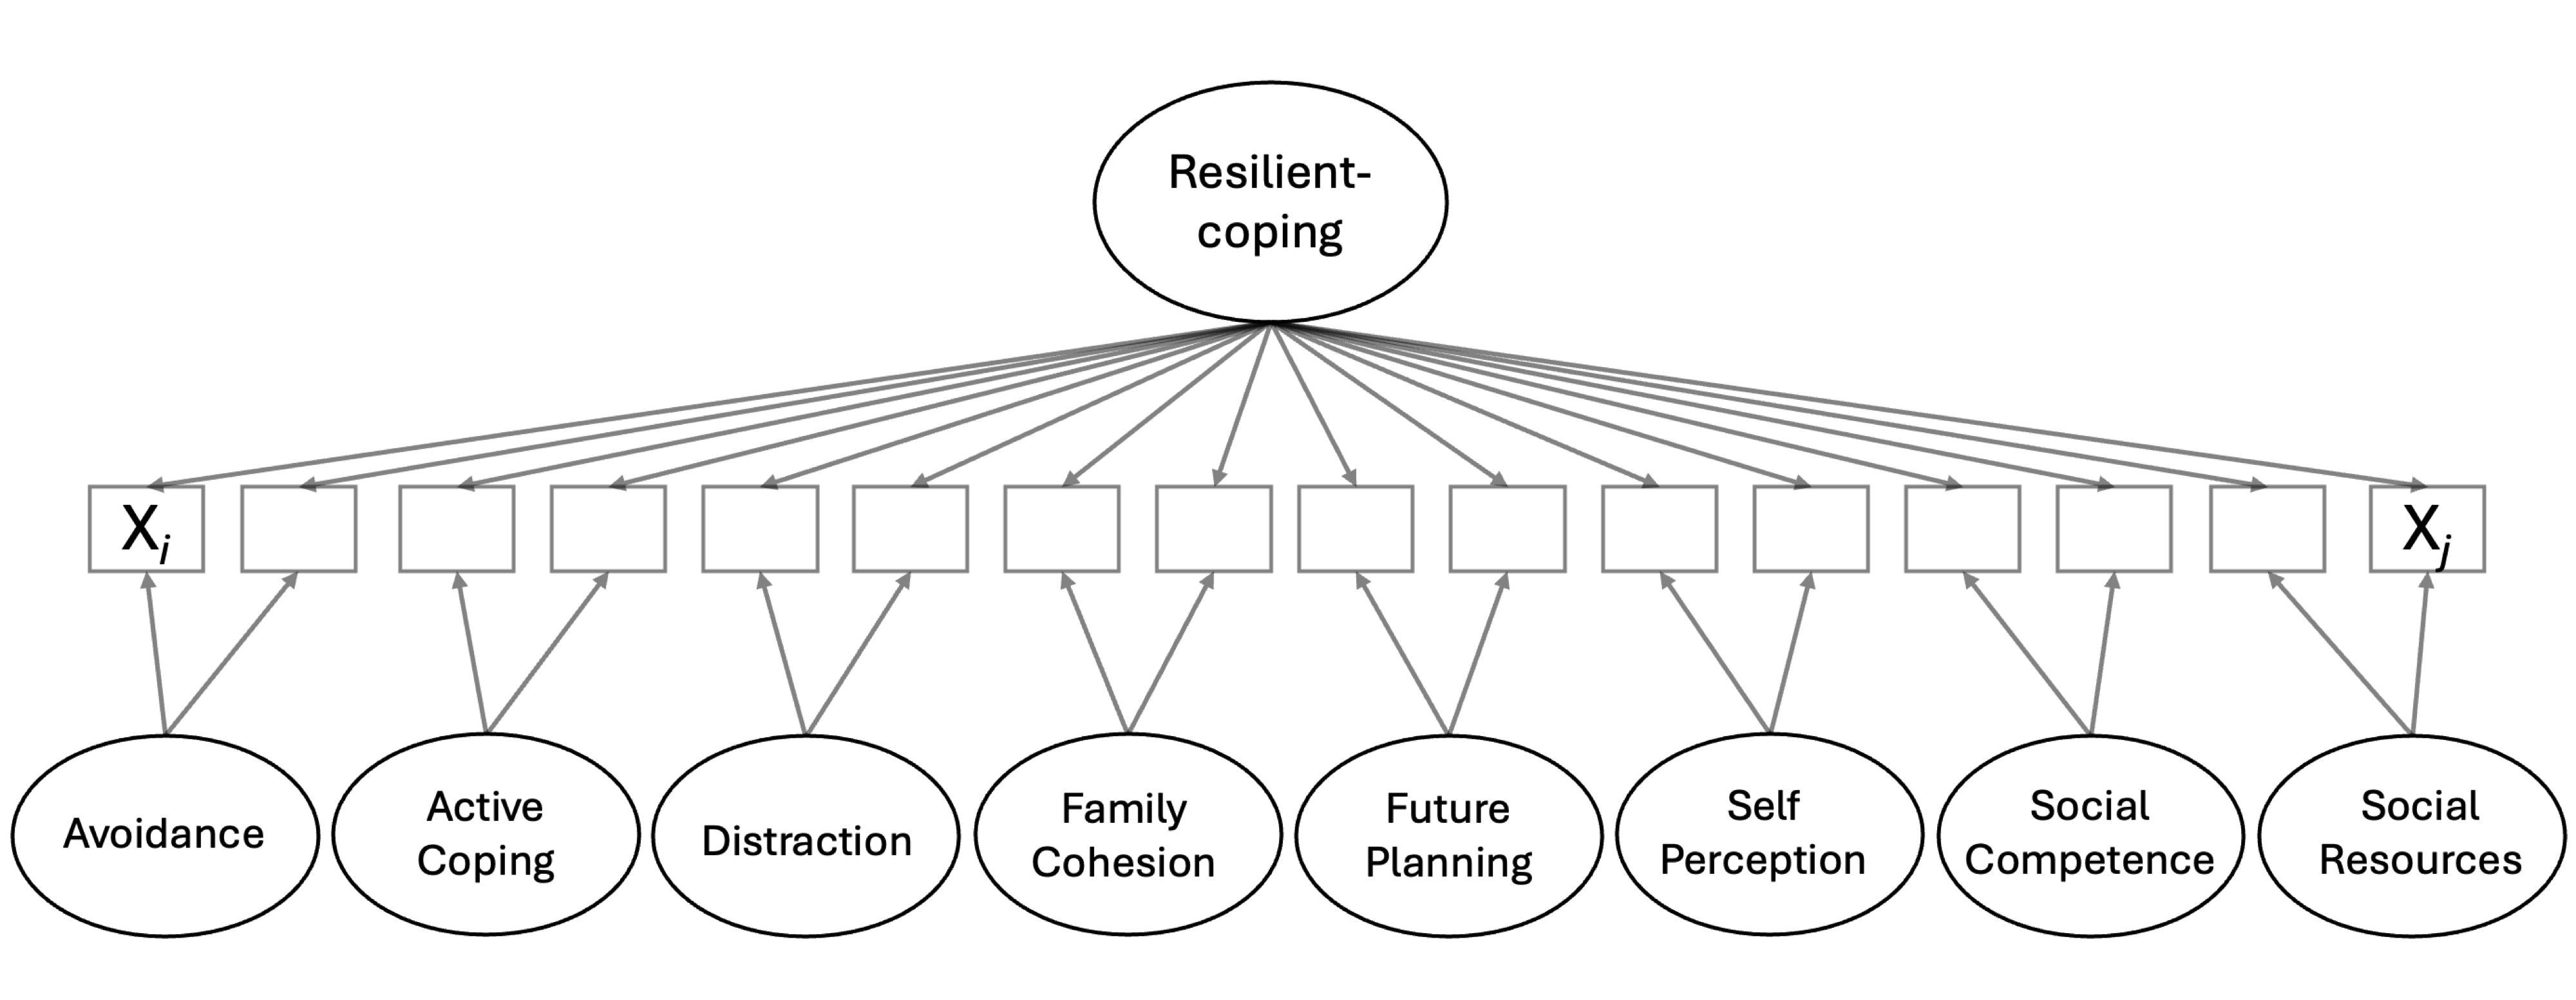
\includegraphics[width=1\linewidth]{sem/sem4_saved_backup} 

}

\end{figure}

\vspace{-30pt}

\emph{Note.} This simplified model illustrates the included items loading on their respective factors. These are the theoretical factors (``-'' denotes a negative factor): \textbf{Avoidance} Behavioral Disengagement (-), Substance Abuse (-), Rejection (-), Self-Blame (-), and Wishful Thinking (-). \textbf{Active Coping} Active Coping and Dealing with Anxiety. \textbf{Distraction} Distraction, Cognitive Restructuring, Physical Effort, and Mental Effort \textbf{Family Cohesion} Family Cohesion. \textbf{Future Planning} Future Planning. \textbf{Self-Perception} Self-Perception, Optimism, Meaning, Purpose and Growth, Positive Thinking, and Acceptance. \textbf{Social Competence} Humor, Instrumental Support, and Planning. \textbf{Social Resources} Social Support and Religion. \normalsize \singlespacing \doublespacing

~~~~~~\textbf{\emph{Item selection procedure.}} In selecting our item pool, we aimed to recover factors beyond a general component. This was accomplished by employing a bifactor model, which allowed us to discern the extent to which the overarching construct versus secondary dimensions account for each item's variance. We favored items with loadings of (\(\lambda_{G}\)) greater than 0.5 for the general factor loading and at least 0.5 for the specific factor. Following Buhner (\citeproc{ref-buhner2006einfuhrung}{2006}), item content is considered particiularly when two competing items within a facet had similar loadings. When specific facets did not reach the loading criteria, we selected the ones with the highest loading on that factor while favoring items with higher loading on the specific factor rather than on the general factor. Also, we considered the theoretical factor and attempt to include as many of them as possible, when loading is suffient enough. Further objectives include ensuring equal items for each factor so that sumscores are applicable.

\subsection{Data analysis}\label{data-analysis}

~~~~~~We implemented IRT paradigma to our polytomous data that follow a 2 parameter logistic Samejimaj. The used algorithm optimizes the maximum likelihood function where each model convergence is reached by a unrestricted iterative process until likelihood change is 0.00010 or below. To compare the performance of different models, we conducted an analysis of variance (ANOVA). A better-performing model was determined using the Akaike information criterion (AIC) and the Bayesian information criterion (BIC), whereby smaller values suggest a better model fit. Following recommendations by Burnham and Anderson (\citeproc{ref-burnham2002model}{2002}), we consider two models to be sufficiently different if the AIC and BIC difference is greater than 10 with a competing model. We assessed construct validity using the multi-trait/multi-method approach as outlined by Campbell and Fiske (\citeproc{ref-Campbell}{1959}). Specifically, we evaluate the alignment with our expected correlative pattern for the RCQ, where measures of the same underlying phenomena (resilience, coping, resilient-coping) correlate in their amount higher with measures of convergence, which in turn, correlate in their amount higher with measures of divergence. We employed Pearson's correlation coefficients for the correlation analysis, interpreting the results based on Cohen's (\citeproc{ref-Cohen}{1988}) conventions. Accordingly, correlation coefficients of \textgreater{} .10 are considered small, coefficients of \textgreater{} .30 are associated with a moderate correlation, and coefficients of .50 or greater represent a large correlation.

~~~~~~The whole data preparation and analysis were conducted on a MacBook Air 2020 M1 using R (v4.4.0; \textcolor{blue}{R Core Team, 2024}) with the following R packages: dplyr (v1.1.4; \textcolor{blue}{Wickham et al., 2023}), forcats (v1.0.0; \textcolor{blue}{Wickham, 2023a}), ggplot2 (v3.5.1; \textcolor{blue}{Wickham, 2016}), ggrepel (v0.9.5; \textcolor{blue}{Slowikowski, 2024}), GPArotation (v2024.3.1; \textcolor{blue}{Bernaards \& Jennrich, 2005}), lattice (v0.22.6; \textcolor{blue}{Sarkar, 2008}), lavaan (v0.6.17; \textcolor{blue}{Rosseel, 2012}), lubridate (v1.9.3; \textcolor{blue}{Grolemund \& Wickham, 2011}), mirt (v1.41; \textcolor{blue}{Chalmers, 2012}), naniar (v1.1.0; \textcolor{blue}{Tierney \& Cook, 2023}), openxlsx (v4.2.5.2; \textcolor{blue}{Schauberger \& Walker, 2023}), papaja (v0.1.2.9000; \textcolor{blue}{Aust \& Barth, 2023}), patchwork (v1.2.0; \textcolor{blue}{Pedersen, 2024}), pheatmap (v1.0.12; \textcolor{blue}{Kolde, 2019}), psych (v2.4.3; \textcolor{blue}{Revelle, 2024}), purrr (v1.0.2; \textcolor{blue}{Wickham \& Henry, 2023}), readr (v2.1.5; \textcolor{blue}{Wickham et al., 2024}), rempsyc (v0.1.7; \textcolor{blue}{Thériault, 2023}), reshape2 (v1.4.4; \textcolor{blue}{Wickham, 2007}), rio (v1.0.1; \textcolor{blue}{Chan et al., 2023}), rstudioapi (v0.16.0; \textcolor{blue}{Ushey et al., 2023}), stringr (v1.5.1; \textcolor{blue}{Wickham, 2023b}), tibble (v3.2.1; \textcolor{blue}{Müller \& Wickham, 2023}), tidyverse (v2.0.0; \textcolor{blue}{Wickham et al., 2019}), tinylabels (v0.2.4; \textcolor{blue}{Barth, 2023}), apaTables (2.0.8; \textcolor{blue}{Stanley, 2021}), and writexl (v1.5.0; \textcolor{blue}{Ooms, 2024}).

\section{Results}\label{results}

\subsection{Exploratory item analysis (pilot study)}\label{exploratory-item-analysis-pilot-study}

~~~~~~\textbf{\emph{Analysis of missing responses.}} In our initial analysis of missing data, we found that 1 percent of all values were missing, with 53 percent of rows containing at least one missing value. Conversely, 47 percent of rows were complete with no missing values. We identified 12 items with particularly high missingness, mostly associated with religion, and some individual items linked to theoretical factors such as self-efficacy (one item), optimism (two items), mental effort (one item), social factor (one item), and moral factor (one item). Further investigation of missingness at the factor level revealed that the religion factor had the highest missingness, exhibiting 5 percent. Other factors with more than 1 percent missing responses include role models, morality, ethics and altruism, mental exhaustion, instrumental support, family cohesion, substance use, and future planning. For subsequent analyses, missing values were replaced with the item mean.

~~~~~~\textbf{\emph{Creation of itemsets.}} In our analysis, we varied multiple exploratory assumptions to create itemsets that perform adequately under these assumptions. The focus was on the magnitude of item loadings across various item constellations rather than model fit. High loadings were particularly interesting as they indicate items strongly related to the underlying factors. Initially, we varied the number of factors from 1 to 26 (based on 26 theoretical factors identified in prior literature analysis) for EFA, PCA, bifactor PCA, and MIRT.

~~~~~~For bifactor PCA, models were adapted with an additional factor, such that factors 3 to 27 corresponded to the assumptions from previous methods. Loadings were quite similar across methods under the same model assumptions. However, under the IRT model, computational demands increased drastically with the number of specified factors due to the iterative procedures optimizing the likelihood function. As the number of factors increased, more parameters had to be estimated, making the optimization process more complex and time-consuming. To meet these computational demands, the maximal iterations to optimize the likelihood function were fixed at 500. Despite this, these models still took several days to compute, and some did not converge. The lack of convergence using quadrature methods may be due to unconstrained items or the inclusion of items that should be removed. Following suggestions by Chalmers (\textcolor{blue}{2012}), we used the quasi-Monte Carlo integration method to stabilize the estimation process with more dimensions. However, the algorithm did not work well when extracting too many dimensions, particularly beyond 22 factors, which we set as the upper limit for the content domain.

~~~~~~Different factor ranges were indicated by both PCA variants, with appropriateness up to 15 factors and EFA up to 20 factors, as these models explained at least 50 percent of the variance. All models are summarized in Figure \ref{fig:myfig23}.

\footnotesize

\begin{figure}[H]
\caption[Model summaries of EFA, PCA, biPCA and MIRT for all inspected itemsets]{Model summaries of EFA, PCA, biPCA and MIRT for all inspected itemsets}\label{fig:myfig23}
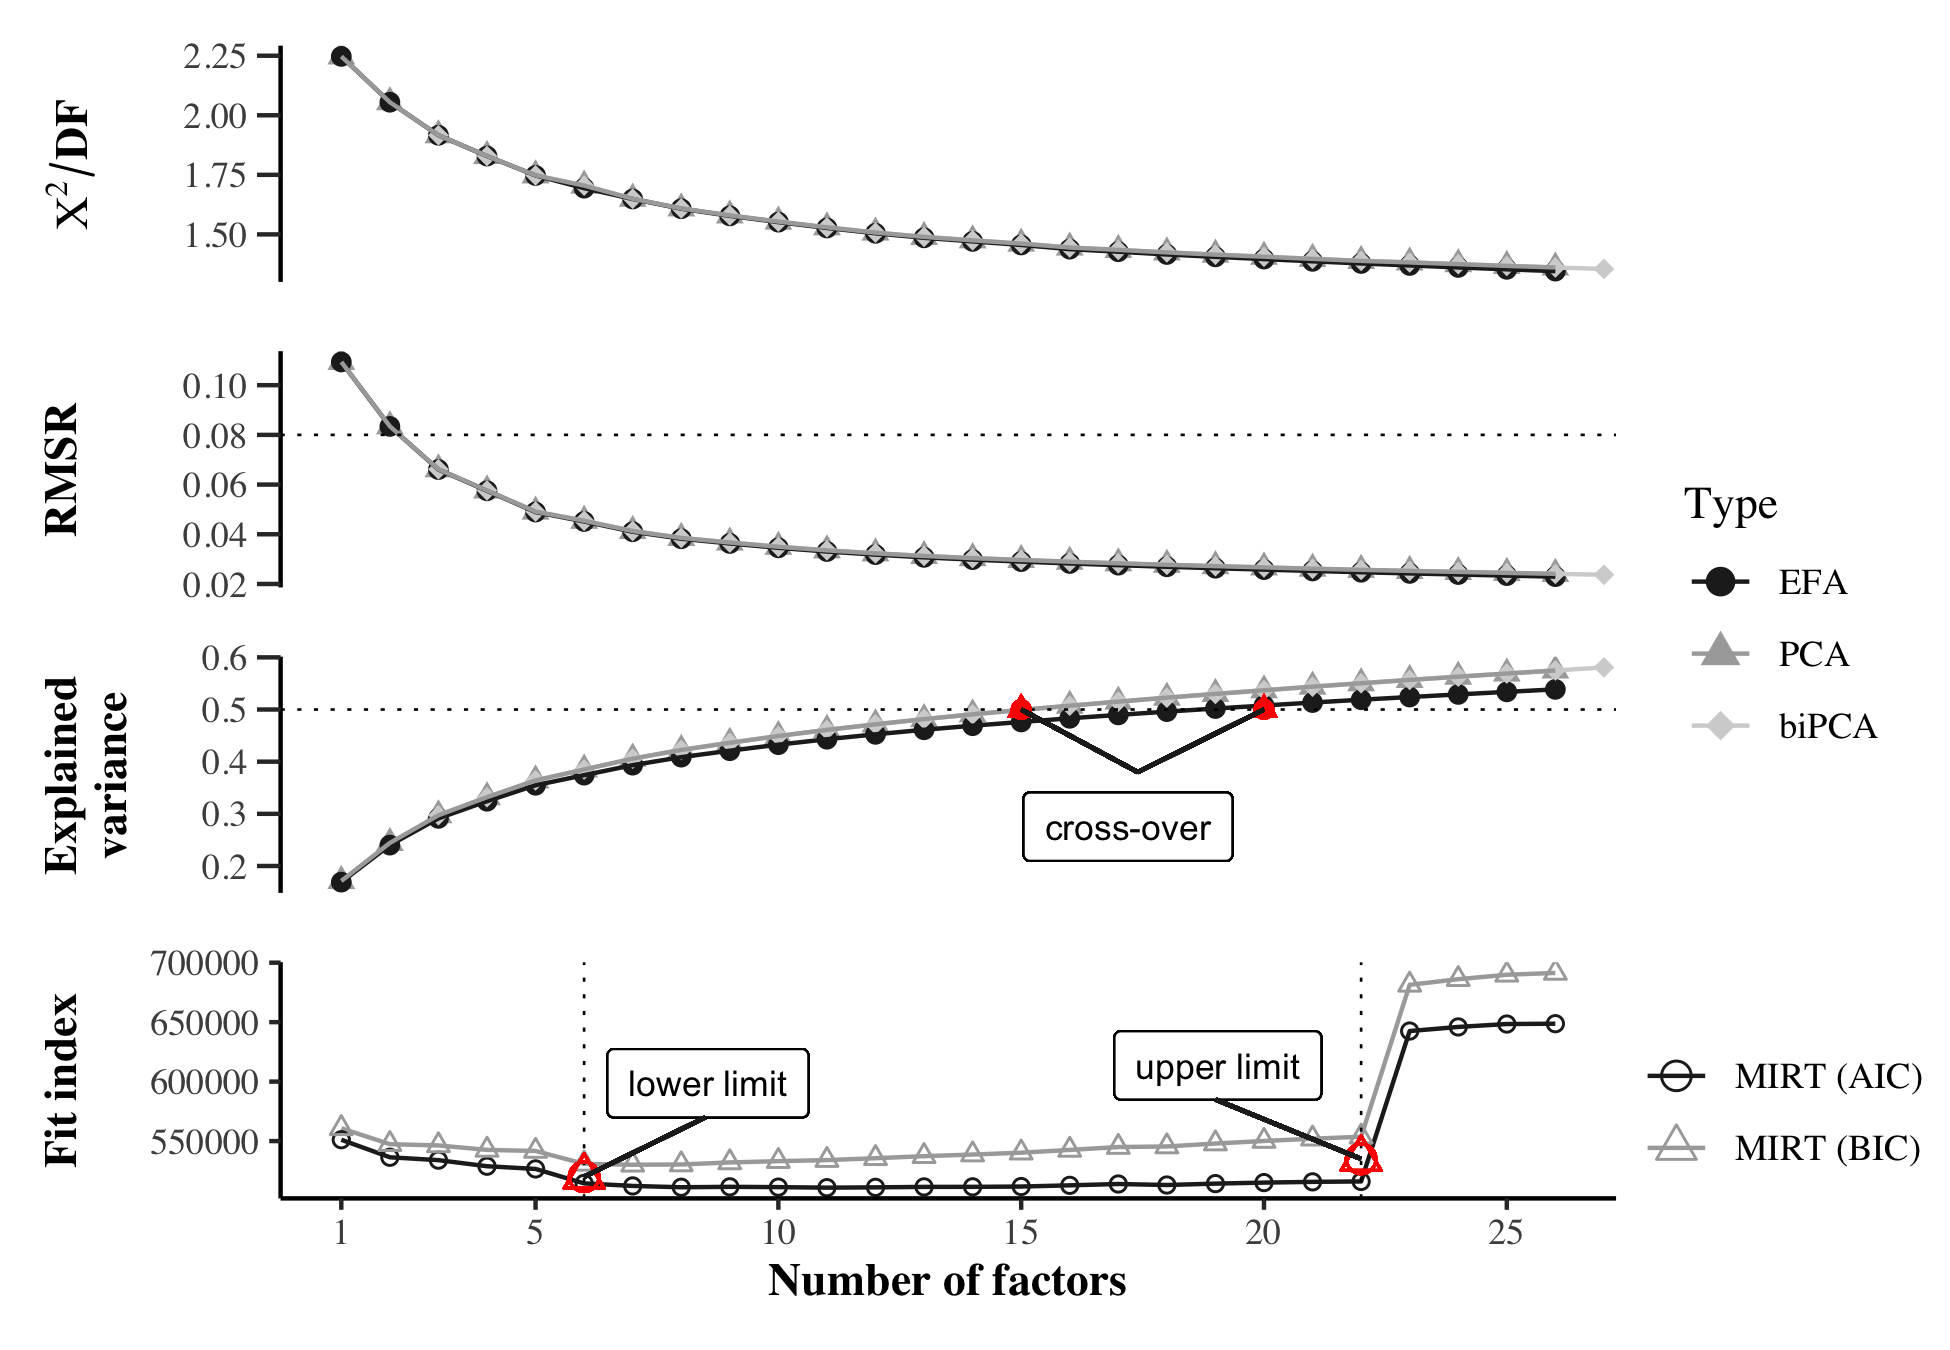
\includegraphics[width=1\linewidth]{2024-06-09_MA_March2024_neuer_verlauf_files/figure-latex/myfig23-1} \end{figure}

\vspace{-30pt}

\noindent  
\emph{Note.} \(\chi^2/df\) = \(\chi^2\) value divided by the degrees of freedom used within the respective model. RMSR = the root mean square residual. VAR = explained variance. Only oblique rotations are displayed, although both oblique and promax rotations yield mostly identical results. \normalsize \singlespacing \doublespacing

~~~~~~Using this method, we identified instances where individual items met the cut-off criteria in one method but not in another, reducing bias in creating subsequent item sets. To reduce the item pool, we applied our item reduction procedure, creating itemsets based on the frequency of incidences where an item's loading was above 0.5. For example, the item with the ID 2''I can now accept things that used to upset me. (translated)'' had a frequency of 109, indicating that the criteria were met in 109 instances. Quantile analysis determined the cutoff for item inclusion, with the 75th percentile serving as the threshold (indicating that a item should be listed in at least 91 instances). We also created an additional itemset for items that frequently did not load below 0.1, thereby identifying 81 such items that frequently did not show low loadings. Additional itemsets were created using correlational results with scales and subscales, including items that correlated highly with measures of the same underlying construct, moderately with convergent validity scales, and low with divergent validity scales. Using these itemsets, we created a baseline of 83 items. To ensure no items with specific conditions were overlooked, items with exceptionally high loadings in any factor solution were added to the reduced itemset, if not already present, expanding the itemset to 105 items.

~~~~~~Finally, we considered missing responses attributable to items answered only by specific subgroups. Factors like religion, substance abuse, and physical effort were examined for their influence on item responses. We computed factor means for these and viewed correlations with convergent measures, supporting the validity claims for factors associated with the unanswered items. Consequently, items with the highest factor loadings and highest item discrimination were included in the reduced itemset, if not already present from previous analyses. This process added one more item, bringing the total to 106 items. We concluded with a final qualitative overlook and decided to remove one item with unclear phrasing and forwarded the remaining 105 items for further analysis and validation. The reduced item pool represents 23 theoretical factors, with items associated with ``moral, ethics, and altruism'', ``structuredness'', and ``role models'' being dropped. The resulting item pool is presented in \hyperref[appendixc]{Appendix C}.

\subsection{Confirmatory factor analysis (present study)}\label{confirmatory-factor-analysis-present-study}

~~~~~~In an initial step, we examined the item correlations using heatmaps. This was crucial to identify and remove items that lacked correlative evidence before confirmatory model testing. Our analysis led to the exclusion of seven items that were associated with religion, substance abuse, and planning. Across two samples, we report that both religion and substance abuse show weak loading patterns. The planning items also underwent scrutiny.

~~~~~~Given that items related to this facett were excluded in prior analyses, the remaining planning item was expected to show limited covariance with other variables. Notably, items of physical effort was also flagged due to its correlation pattern. However, the correlations were less severe, and unlike the other items, items were supported in prior exploratory analysis. Moreover, given its conceptual relevance to the `distraction' factor (as per Ayers and colleagues), we retained the two items related to physical effort. Consequently, the CFA was conducted on the remaining 98 items, representing 20 theoretical factors. Further results regard the performance of models.

~~~~~~All models tested were superior to the baseline models (resilience items used as reference factor, \emph{AIC} = 355,984, \emph{BIC} = 359,702); coping items used as reference factor, \emph{AIC} = 356,179, \emph{BIC} = 359,907) and the two-factor model (\emph{AIC} = 353,011, \emph{BIC} = 356,982), supporting the multidimensional nature of our data. Between the two baseline models, data suggests a stronger emphasis on the resilience/coping aspect among the general factor. Among the competing models, the Ayers and colleagues' model (\emph{AIC} = 350,184, \emph{BIC} = 354,155) demonstrated superior performance than the Kaiser and colleagues model (\emph{AIC} = 349,998, \emph{BIC} = 353,969), as indicated by the information criteria metrics. Our preferred 8D solution, Model 5 (\emph{AIC} = 348,691, \emph{BIC} = 352,663), showed a slight advantage over the 5D and 6D solution. In general, simpler models (i.e., less factors) are to be favored, however we consider the differences in both AIC and BIC to be substantial enough to favor the 8D solution over the 5D solution (\citeproc{ref-burnham2002model}{Burnham \& Anderson, 2002}). As this analysis indicated, the eight-dimensional factor solution outperformed its competing alternatives, and subsequent item selection is therefore based on Model 5.

~~~~~~\textbf{\emph{Final item selection.}} After a thorough item selection process, we arrived at a final set of 30 items. Notably, the diverse theoretical factors we initially assigned to the factors differ from the final set. However, the factors are still present for \emph{Avoidance} (behavioral disengagement, rejection, self-blame, wishful thinking), \emph{Distraction} (distraction, physical effort), and \emph{Self-Perception} (acceptance, meaning, purpose, and growth, optimism, positive thinking).

~~~~~~The factors are only partially present for \emph{Active Coping}, where \emph{dealing with anxiety} remains as the theoretical factor. In contrast, the factors are not present for \emph{Family Cohesion}, \emph{Future Planning}, \emph{Social Competence}, and \emph{Social Resources}. Additionally, for \emph{Social Competence}, only items with the theoretical factor humor remained.

~~~~~~To conclude the development process, we reran the model with the selected items and further present the RCQ. Its dimensional structure has a 1st to 2nd (\emph{Resilient-coping} to \emph{Family Cohesion}) eigenvalue ratio of 8.40 to 2.10, indicating a strong emphasis on the general factor. Specifically, 28 percent of the variance is explained by the general factor, while the variance for the specific factors varie from 7 to 2 percent. Following the eigenvalues-greater-than-one criterion, the second eigenvalue is indicative of sufficient variance accounted for by this factor. This is also true for \emph{Distraction} (2.01), \emph{Avoidance} (1.32), \emph{Social Competence} (1.15), and \emph{Social Resources} (1.11). However, the factors \emph{Future Planning} (0.81), \emph{Active Coping} (0.71), and \emph{Self-Perception} (0.68) did not reach the eigenvalue criterion.

\newpage
\phantomsection

\label{table1}

\begin{lltable}

\begin{TableNotes}[para]
\normalsize{\textit{Note.} {\justifying Associated labels are: $\lambda_1$: Avoidance, $\lambda_2$: Self-Perception, $\lambda_3$: Future Planning, $\lambda_4$: Social Competence, $\lambda_5$: Family Cohesion,\\ $\lambda_6$: Social Resources, $\lambda_7$: Distraction, and $\lambda_8$: Active Coping. The item response function models the probability of endorsing a \\particular response category ({\textcolor{blue}{de Ayala, 2022}}). Samejima ({\textcolor{blue}{1968}}) assumes a logistic function of the difference in the person's ability level ($\theta$) based on item discrimination ($a_i$) and item difficulty ($b_i$) in the 2PL model. Here, $a_i$ indicates how well an item discrimi-\\nates between different levels of the trait, and $b_i$ represents the difficulty parameter for an item, indicating where the response prob-\\ability is 50\%.}}
\end{TableNotes}

\footnotesize{

\begin{longtable}{ccccccccccccccccccc}\noalign{\getlongtablewidth\global\LTcapwidth=\longtablewidth}
\caption{\label{tab:ladu4}Discrimination, difficulty and item parameters for the Bifactor MIRT Model}\\
\toprule
 & \multicolumn{9}{c}{Standardized factor loadings (8D bifactor)} & \multicolumn{2}{c}{Discrimination} & \multicolumn{6}{c}{Difficulty}  &\\
\cmidrule(r){2-10} \cmidrule(r){11-12} \cmidrule(r){13-18}
Item & \multicolumn{1}{c}{$\lambda_{G}$} & \multicolumn{1}{c}{$\lambda_{S1}$} & \multicolumn{1}{c}{$\lambda_{S2}$} & \multicolumn{1}{c}{$\lambda_{S3}$} & \multicolumn{1}{c}{$\lambda_{S4}$} & \multicolumn{1}{c}{$\lambda_{S5}$} & \multicolumn{1}{c}{$\lambda_{S6}$} & \multicolumn{1}{c}{$\lambda_{S7}$} & \multicolumn{1}{c}{$\lambda_{S8}$} & \multicolumn{1}{c}{$a_{G}$} & \multicolumn{1}{c}{$a_{S}$} & \multicolumn{1}{c}{$d_{1}$} & \multicolumn{1}{c}{$d_{2}$} & \multicolumn{1}{c}{$d_{3}$} & \multicolumn{1}{c}{$d_{4}$} & \multicolumn{1}{c}{$d_{5}$} & \multicolumn{1}{c}{$d_{6}$} & \multicolumn{1}{c}{$h^2$}\\
\midrule
\endfirsthead
\caption*{\normalfont{Table \ref{tab:ladu4} continued}}\\
\toprule
 & \multicolumn{9}{c}{Standardized factor loadings (8D bifactor)} & \multicolumn{2}{c}{Discrimination} & \multicolumn{6}{c}{Difficulty}  &\\
\cmidrule(r){2-10} \cmidrule(r){11-12} \cmidrule(r){13-18}
Item & \multicolumn{1}{c}{$\lambda_{G}$} & \multicolumn{1}{c}{$\lambda_{S1}$} & \multicolumn{1}{c}{$\lambda_{S2}$} & \multicolumn{1}{c}{$\lambda_{S3}$} & \multicolumn{1}{c}{$\lambda_{S4}$} & \multicolumn{1}{c}{$\lambda_{S5}$} & \multicolumn{1}{c}{$\lambda_{S6}$} & \multicolumn{1}{c}{$\lambda_{S7}$} & \multicolumn{1}{c}{$\lambda_{S8}$} & \multicolumn{1}{c}{$a_{G}$} & \multicolumn{1}{c}{$a_{S}$} & \multicolumn{1}{c}{$d_{1}$} & \multicolumn{1}{c}{$d_{2}$} & \multicolumn{1}{c}{$d_{3}$} & \multicolumn{1}{c}{$d_{4}$} & \multicolumn{1}{c}{$d_{5}$} & \multicolumn{1}{c}{$d_{6}$} & \multicolumn{1}{c}{$h^2$}\\
\midrule
\endhead
\phantomsection\label{behav_1_133_r}\hyperref[behav_1_133_r]{\textcolor{blue}{1}} & \cellcolor{lightgray} 0.56 & \cellcolor{lightgray} 0.68 &  &  &  &  &  &  &  & 2.02 & 2.42 & 8.15 & 6.42 & 4.61 & 2.84 & 0.98 & -1.65 & 0.77\\
\phantomsection\label{behav_1_129_r}\hyperref[behav_1_129_r]{\textcolor{blue}{2}} & \cellcolor{lightgray} 0.55 & \cellcolor{lightgray} 0.55 &  &  &  &  &  &  &  & 1.48 & 1.49 & 5.55 & 4.04 & 2.60 & 1.29 & -0.15 & -2.44 & 0.60\\
\phantomsection\label{behav_1_132_r}\hyperref[behav_1_132_r]{\textcolor{blue}{3}} & \cellcolor{lightgray} 0.50 & 0.49 &  &  &  &  &  &  &  & 1.19 & 1.18 & 4.92 & 3.43 & 1.94 & 0.45 & -0.81 & -2.71 & 0.49\\
\phantomsection\label{wunsc_1_154_r}\hyperref[wunsc_1_154_r]{\textcolor{blue}{4}} & 0.35 & 0.35 &  &  &  &  &  &  &  & 0.69 & 0.69 & 3.86 & 2.83 & 1.95 & 1.23 & 0.68 & -0.33 & 0.25\\
\phantomsection\label{selbv_1_198_r}\hyperref[selbv_1_198_r]{\textcolor{blue}{5}} & \fbox{\cellcolor{white} 0.17} & 0.33 &  &  &  &  &  &  &  & 0.30 & 0.61 & 2.36 & 1.46 & 0.61 & -0.05 & -0.41 & -1.02 & 0.14\\
\phantomsection\label{ableh_2_081_r}\hyperref[ableh_2_081_r]{\textcolor{blue}{6}} & 0.32 & \fbox{\cellcolor{white} 0.27} &  &  &  &  &  &  &  & 0.60 & 0.52 & 3.34 & 2.53 & 1.54 & 1.02 & 0.39 & -0.78 & 0.18\\
\phantomsection\label{sinnz_2_312}\hyperref[sinnz_2_312]{\textcolor{blue}{7}} & \cellcolor{lightgray} 0.58 &  & \cellcolor{lightgray} 0.56 &  &  &  &  &  &  & 1.66 & 1.62 & 4.32 & 2.76 & 1.54 & -0.03 & -2.13 & -3.83 & 0.65\\
\phantomsection\label{sinnz_1_300}\hyperref[sinnz_1_300]{\textcolor{blue}{8}} & \cellcolor{lightgray} 0.63 &  & 0.44 &  &  &  &  &  &  & 1.68 & 1.19 & 5.12 & 3.52 & 2.34 & 1.01 & -0.65 & -2.41 & 0.59\\
\phantomsection\label{posit_1_167}\hyperref[posit_1_167]{\textcolor{blue}{9}} & \cellcolor{lightgray} 0.78 &  & 0.32 &  &  &  &  &  &  & 2.52 & 1.04 & 6.38 & 4.54 & 3.19 & 1.57 & -0.89 & -3.15 & 0.72\\
\phantomsection\label{selbw_2_325}\hyperref[selbw_2_325]{\textcolor{blue}{10}} & \cellcolor{lightgray} 0.81 &  & \fbox{\cellcolor{white} 0.15} &  &  &  &  &  &  & 2.45 & 0.45 & 6.97 & 5.28 & 3.91 & 2.25 & -0.24 & -2.93 & 0.68\\
\phantomsection\label{akzep_3_019}\hyperref[akzep_3_019]{\textcolor{blue}{11}} & \cellcolor{lightgray} 0.60 &  & \fbox{\cellcolor{white} 0.14} &  &  &  &  &  &  & 1.31 & 0.31 & 4.15 & 3.34 & 2.27 & 1.13 & -0.45 & -2.29 & 0.39\\
\phantomsection\label{optim_2_211_r}\hyperref[optim_2_211_r]{\textcolor{blue}{12}} & \cellcolor{lightgray} 0.73 &  & \fbox{\cellcolor{white} 0.12} &  &  &  &  &  &  & 1.84 & 0.30 & 5.03 & 3.81 & 2.59 & 1.38 & -0.24 & -2.30 & 0.55\\
\phantomsection\label{zukun_1_339}\hyperref[zukun_1_339]{\textcolor{blue}{13}} & \cellcolor{lightgray} 0.60 &  &  & \cellcolor{lightgray} 0.72 &  &  &  &  &  & 2.90 & 3.52 & 8.14 & 6.00 & 4.28 & 2.19 & -1.04 & -4.51 & 0.88\\
\phantomsection\label{zukun_2_347}\hyperref[zukun_2_347]{\textcolor{blue}{14}} & \cellcolor{lightgray} 0.76 &  &  & 0.41 &  &  &  &  &  & 2.55 & 1.39 & 6.84 & 5.27 & 3.85 & 1.92 & -0.25 & -3.15 & 0.74\\
\phantomsection\label{zukun_2_344}\hyperref[zukun_2_344]{\textcolor{blue}{15}} & \cellcolor{lightgray} 0.50 &  &  & 0.34 &  &  &  &  &  & 1.07 & 0.72 & 3.68 & 2.40 & 1.55 & 0.59 & -0.66 & -2.08 & 0.37\\
\phantomsection\label{humor_1_082}\hyperref[humor_1_082]{\textcolor{blue}{16}} & \cellcolor{lightgray} 0.58 &  &  &  & \cellcolor{lightgray} 0.71 &  &  &  &  & 2.49 & 3.01 & 7.83 & 6.60 & 4.80 & 2.91 & 0.19 & -2.91 & 0.84\\
\phantomsection\label{humor_1_087}\hyperref[humor_1_087]{\textcolor{blue}{17}} & 0.48 &  &  &  & \cellcolor{lightgray} 0.57 &  &  &  &  & 1.23 & 1.47 & 5.09 & 4.55 & 3.55 & 2.49 & 1.14 & -0.86 & 0.56\\
\phantomsection\label{humor_1_085_r}\hyperref[humor_1_085_r]{\textcolor{blue}{18}} & 0.40 &  &  &  & \cellcolor{lightgray} 0.56 &  &  &  &  & 0.94 & 1.32 & 3.94 & 2.41 & 1.20 & 0.33 & -0.75 & -2.29 & 0.48\\
\phantomsection\label{famil_1_373}\hyperref[famil_1_373]{\textcolor{blue}{19}} & 0.41 &  &  &  &  & \cellcolor{lightgray} 0.90 &  &  &  & 4.28 & 9.30 & 18.69 & 14.65 & 11.83 & 8.49 & 4.44 & -0.71 & 0.97\\
\phantomsection\label{famil_1_371}\hyperref[famil_1_371]{\textcolor{blue}{20}} & 0.37 &  &  &  &  & \cellcolor{lightgray} 0.80 &  &  &  & 1.32 & 2.84 & 6.40 & 5.03 & 4.09 & 2.65 & 1.11 & -0.98 & 0.77\\
\phantomsection\label{famil_1_378}\hyperref[famil_1_378]{\textcolor{blue}{21}} & 0.44 &  &  &  &  & \cellcolor{lightgray} 0.79 &  &  &  & 1.75 & 3.16 & 7.15 & 5.42 & 4.26 & 2.82 & 1.03 & -1.23 & 0.82\\
\phantomsection\label{sozia_1_355}\hyperref[sozia_1_355]{\textcolor{blue}{22}} & 0.37 &  &  &  &  &  & \cellcolor{lightgray} 0.70 &  &  & 1.03 & 1.98 & 5.60 & 4.09 & 3.20 & 2.18 & 0.58 & -1.09 & 0.63\\
\phantomsection\label{sozia_1_038}\hyperref[sozia_1_038]{\textcolor{blue}{23}} & \cellcolor{lightgray} 0.54 &  &  &  &  &  & \cellcolor{lightgray} 0.57 &  &  & 1.47 & 1.57 & 5.38 & 4.26 & 3.33 & 2.02 & 0.44 & -1.51 & 0.62\\
\phantomsection\label{sozia_1_354}\hyperref[sozia_1_354]{\textcolor{blue}{24}} & \cellcolor{lightgray} 0.58 &  &  &  &  &  & \cellcolor{lightgray} 0.53 &  &  & 1.59 & 1.47 & 5.22 & 4.77 & 4.04 & 2.73 & 1.01 & -0.92 & 0.62\\
\phantomsection\label{physi_1_264}\hyperref[physi_1_264]{\textcolor{blue}{25}} & \fbox{\cellcolor{white} 0.22} &  &  &  &  &  &  & \cellcolor{lightgray} 0.93 &  & 1.29 & 5.58 & 7.28 & 4.77 & 3.08 & 1.97 & -0.50 & -3.27 & 0.92\\
\phantomsection\label{physi_1_263}\hyperref[physi_1_263]{\textcolor{blue}{26}} & \fbox{\cellcolor{white} 0.25} &  &  &  &  &  &  & \cellcolor{lightgray} 0.92 &  & 1.33 & 4.98 & 5.22 & 3.36 & 2.09 & 1.01 & -0.67 & -2.41 & 0.90\\
\phantomsection\label{ablen_1_048}\hyperref[ablen_1_048]{\textcolor{blue}{27}} & 0.39 &  &  &  &  &  &  & \cellcolor{lightgray} 0.54 &  & 0.88 & 1.23 & 2.80 & 1.92 & 1.27 & 0.47 & -0.66 & -2.05 & 0.44\\
\phantomsection\label{umgan_1_221}\hyperref[umgan_1_221]{\textcolor{blue}{28}} & \cellcolor{lightgray} 0.52 &  &  &  &  &  &  &  & \cellcolor{lightgray} 0.72 & 1.94 & 2.70 & 6.95 & 5.08 & 3.17 & 0.97 & -1.84 & -4.62 & 0.79\\
\phantomsection\label{umgan_1_222}\hyperref[umgan_1_222]{\textcolor{blue}{29}} & \cellcolor{lightgray} 0.51 &  &  &  &  &  &  &  & 0.34 & 1.09 & 0.72 & 4.37 & 3.10 & 2.07 & 0.98 & -0.66 & -2.23 & 0.37\\
\phantomsection\label{aktiv_1_180}\hyperref[aktiv_1_180]{\textcolor{blue}{30}} & \cellcolor{lightgray} 0.65 &  &  &  &  &  &  &  & \fbox{\cellcolor{white} 0.27} & 1.57 & 0.65 & 4.20 & 2.64 & 1.35 & -0.60 & -2.14 & -3.92 & 0.50\\
\bottomrule
\addlinespace
\insertTableNotes
\end{longtable}

}

\end{lltable}

\newpage

~~~~~~\textbf{\emph{Reliability estimates.}} In situations where data follow a bifactor structure, the Omega Hierarchical (\(\upomega_{H}\)) is useful for assessing reliability. Unlike other reliability measures like Cronbach's alpha and omega, which consider all sources of common variance, \(upomega_{H}\) focuses explicitly on the proportion of variance in total scores attributed to a single overarching factor, thereby treating variability in scores due to group factors as measurement error (\citeproc{ref-rodriguez_evaluating_2016}{Rodriguez et al., 2016}). This makes it particularly useful for understanding how much of the variability in scores can be explained by this general factor: \[ \upomega_H = \frac{ ( \sum \lambda_{\text{general factor}})^2}{( \sum \lambda_{\text{general factor}})^2 + \sum_{j=1}^{k} (\sum \lambda_{\text{specific factor}_j})^2 + \sum(1-h^2)}. \]\\
\strut ~~~~~~In this formula \(\lambda_{\text{general factor}}\) denotes the variance attributed to the general factor, and \(\lambda_{\text{specific factors}_j}\) signifies the residual variances of the observed variables. This concept can be extended to subscales by calculating the unique variance associated with each group factor after removing the variance linked to a general factor. This extension is captured through the coefficient Omega Hierarchical Subscale (\(\upomega_{HS}\)), which serves as an indicator of the reliability of a given subscale score while accounting for the general factor's influence (Reise et al., 2013, cited in \citeproc{ref-rodriguez_evaluating_2016}{Rodriguez et al., 2016}).

~~~~~~OmegaHS for a given subscale \(i\) is determined using the following formula: \[ \upomega_{HS} = \frac{(\sum \lambda_{\text{ specific factor}_i})^2}{(\sum_{i=1}^{i=k} \lambda_{\text{general factor}})^2 + (\sum \lambda_{\text{specific factor}_i})^2 + \sum_{i=1}^{i=k}(1-h^2)}. \]\\
\strut ~~~~~~For the FRC, we report a total omegaH of .84, indicating that 84percent of the variance of unit-weighted total scores can be attributed to the individual differences on the general factor. Following recommendations by Rodriguez et al. (\citeproc{ref-rodriguez_evaluating_2016}{2016}), we compare the difference between omega and omegaH (96 percent - 84\%), which indicates, that 12 percent of the reliable variance in total scores can be attributed to the multidimensionality caused by the group factors. The remaining 4percent is due to a estimated random error. For the subscales avoidance, self-perception, future planning, social competence, family cohesion, social resources, distraction, and active coping, omegaH coefficients are calculated as .43, .13, .33, .51, .76, .50, .80 and .30, respectively.

~~~~~~\textbf{\emph{Validity assessment.}} The construct validity of the RCQ was assessed by examining the correlations between the RCQ and various related and unrelated measures. The highest correlations were observed with instruments measuring the same underlying phenomena, indicating strong convergent validity. Specifically, the RCQ showed high correlations with resilience (\(r_{\text{RS-11}}\) = .80), coping (\(r_{\text{MCCS}}\) = .74), and resilient-coping (\(r_{\text{BRCS}}\) = .65). Similarly, closely related constructs such as satisfaction with life (\(r_{\text{SWLS}}\) = .61), general self-efficacy (\(r_{\text{GSE}}\) = .64), negative emotionality (\(r_{\text{Negative Emotionality}}\) = -.59), and extraversion (\(r_{\text{Extravision}}\) = .56) also demonstrated high and sufficient correlations, further supporting the construct validity of the RCQ. In contrast, the RCQ showed relatively high correlations with the personality dimensions of conscientiousness (\(r_{\text{Conscientiousness}}\) = .51), agreeableness (\(r_{\text{Agreeableness}}\) = .51), and openness to experience (\(r_{\text{Openness}}\) = .43), which are considered unrelated measures. However, these correlations were still lower than those observed with related measures. Additional measures of divergence indicated minimal to moderate relations of the RCQ with perceived political self-efficacy (\(r_{\text{P-PSE}}\) = .18) and general procrastination (\(r_{\text{GPS-K}}\) = -.33). These findings are consistent with the expected correlative pattern, providing strong evidence of the validity of the RCQ. All correlative results are displayed in \hyperref[appendixb]{Appendix B}.

\section{General discussion}\label{general-discussion}

In this thesis, we aimed to investigate the dimensionality of resilience and coping within a German-speaking population, leading to the development of the RCQ. Our findings indicate that a combined bifactor model better represents the RCQ, addressing the limitation of missing coping aspects within dimensional solutions of resilience, and vice versa, focusing on all aspects contributing to a positive adaptation to adversity. We adopted an exploratory approach in which we allowed the content domain to influence the identification of relevant aspects and fited our findings to existing models in the literature using our item bank. As Kaplan (1999) stated, ``we must continually re-examine exciting ideas to make sure that they are worthy of the intellectual resources focused upon them (cited in \citeproc{ref-manyena_concept_2006}{Manyena, 2006, p. 440}).'' Therefore, instead of adding new dimensional labels, we emphasized the significant contributions already made in this field.

Regarding our aims, we demonstrated that the construct at hand is in fact multidimensional, aligning with existing literature that highlights their importance in psychological assessments (criterion 1). Similarly, coping components are also represented in a multidimensional manner, ensuring a balanced and thorough assessment of both resilience factors and coping mechanisms (criterion 2). However, it should be considered that the separation between resilience and coping in our approach had a practical purpose to allow a broad content domain, but are not strictly to be separated as two different concepts (alighning with Leipold and Greve (\citeproc{ref-leipold_greve_2009}{2009}) perspective). For instance, religion and other social factors were present in most of our literature models regarding both resilience and coping, further highlighting the conceptual and empirical overlap.

\subsection{Dimensionality of the RCQ}\label{dimensionality-of-the-rcq}

~~~~~~The claim of multidimensionality was reassured in the pilot and present study. As intended, unsuitable theoretical factors were dropped along the way. An explanation for their exclusion was not solely based on evidence at the factor level but also at the item level. Specifically, factors related to religion did not manifest in our approach. This could be due to non-responsiveness to these items as religious individuals seem not to be included in our convenience sample. This could also indicate the general population's hesitance to answer such items, or due to our sample consisting largely of academic individuals. We believe that other populations with different national contexts, such as the USA, where religion has a more significant influence, might show different results, shown by Southwick and Charney (\citeproc{ref-southwick2018resilience}{2018}). Besides that, the theoretical factor substance abuse did not replicate in our sample, also likely due to the non-responsiveness. In this regard, it is worth mentioning that a test practitioner explained hesitance in including a measure with such sensitive information, specifically in the organizational context. As this aligns with our empirical findings such items are not further maintained.

~~~~~~Further results regard the integration of five factors from Kaiser and colleagues' model and three factors from Ayers and colleagues' model. The sixth factor used by Kaiser and colleagues reflects structuredness, which was not imported into the factorial structure, as our pilot study only passed on one item of our theoretical factor planning, which we think aligns with the dimension identified. As it was additionally unrelated to other validation scales, we dropped this factor entirely. However, similar problems described by Kaiser and colleagues were encountered with other dimensions that lacked sufficient loadings or were not manifested sufficiently. We reported this for items associated with factors of Active Coping, Self-Perception, and Avoidance. On the factor level, we reported support for five of our eight-dimensional bifactor model. Lower eigenvalues for the three insufficient factors could be attributed to the relatively small number of items per factor. In this regard, the lowest eigenvalue for \emph{Self-Perception} could also be explained conceptually; remaining items of the theoretical factors acceptance, meaning, purpose, and growth, optimism, and positive thinking could be misspecified under its common facet, which is reflected by their in turn higher loading on the general factor. Such an explanation is also plausible for \emph{Active Coping} as we included the theoretical factor dealing with anxiety to it.

\subsection{Reliability- and validity-statement for the RCQ}\label{reliability--and-validity-statement-for-the-rcq}

~~~~~~Reliability estimates for the RCQ show a acceptable amount of variance that could be attributed to individual differences on the general factor. After accounting for the general component, we view that there is enough variance left to identifie specific group factors. While for most factors, sufficient reliability estimates are presented, we see problems with the factors self-perception, future planning, and active coping. No sufficient reliability can be estimated for these scales, which is also reflected in their loadings. This could be an indication that further item or factor adaptations should be made. This could include reassigning or rephrasing these items in ongoing research. While these problems are present, we see the lack of these reliability estimation in combination with the content validity of their theoretical factor from our conceptual work. If these items continue to show practical use, it might be a functional problem of the model representation, which could be fixed with proper constraints, which in turn need to be further empirically evaluated.

~~~~~~Regarding validity statements, study results indicate strong associations with measures of the same underlying phenomena as well as with convergent measures, consistent with Campbell and Fiske's criteria for construct validity. However, individual correlative indices were higher than expected. While we were surprised by the unexpectedly high correlative indices for agreeableness and consciousness, Campbell and Fiske suggest that these associations need not be zero but should be lower than their higher-level associations (i.e., convergent measures). Additionally, minimal to moderate correlations with constructs like perceived political self-efficacy and general procrastination support the RCQ's divergent validity. Despite some unexpected findings, the overall strong first and second level correlations provide robust evidence of the RCQ's validity. Future studies may need to adjust validation strategies, but current results affirm the RCQ's validity.

~~~~~~\textbf{\emph{Limitations and future outlook.}} Adopting a bifactor model allowed us to model a general factor of resilient-coping while focusing on the additional factors specific to our models. However, the bifactor model has its controversies, as noted by Bonifay et al. (\citeproc{ref-bonifay2017}{2017}), particularly regarding the interpretation of primary and secondary dimensions and its tendency to fit well into almost any data pattern. Additionally, we forced model convergence in the present study, which raises concerns about the appropriateness of the number of iterations used for convergence. Despite this, we believe there is enough theoretical support to justify forcing convergence, which may also be influenced by the number of items used in this study.

~~~~~~Further challenges regard the MIRT indices and model identification. The sparseness and missing constraints raised concerns about the reliability of the IRT indices, prompting further investigation into alternative structures. Moreover, we encountered issues of test length and participant dropout, especially in the pilot study, which underscores the need for a different sampling method when dealing with a high number of variables to reduce the burden on test-takers (see e.g., \citeproc{ref-hansen_methodology_2014}{Hansen et al., 2014} for such example). Additionally, our study faced challenges in operationalizing subjective life events and experiences into objective ratings, also reported by Connor-Smith et al. (\citeproc{ref-connor-smith_responses_2000}{2000}). This was particularly evident for items associated with the factors of morality, ethics, altruism, structuredness, and role models, leading to their exclusion due to a lack of meaningful loadings, that raise concerns about the alignment of an item's intent and its actual measurement. Future research should include item revisions, more extensive model testing, and exploration of the temporal precedence of coping or resilience. Examining specific target groups (e.g., highly resilient individuals) would be also particularly informative in this regard. These future directions will provide a more nuanced understanding of the broader functionalities of the RCQ and its dimensionality.

~~~~~~\textbf{\emph{Conclusion.}} This thesis underscores the complexity of measuring resilience and coping and highlights the potential of the RCQ as a tool for advancing our understanding of a unified construct with a multidimensional lense. By addressing the limitations of existing models and proposing a combined approach, we contribute to the ongoing dialogue within the psychological community and lay an alternative groundwork for future research in this area. While postulating a dimensional structure for the RCQ, we do not conclude with a set in stone dimensional postulation and instead aim to further investigate until a suiting empirical structure for resilient-coping is identified. As we continue to explore this domain, the RCQ offers additional perspectives for understanding and supporting individuals in their journey through adversity.

\newpage

\section{References}\label{references}

\footnotesize

\phantomsection\label{refs}
\begin{CSLReferences}{1}{0}
\bibitem[\citeproctext]{ref-agaibi_wilson_2005}
Agaibi, C. E., \& Wilson, J. P. (2005). Trauma, PTSD, and resilience: A review of the literature. \emph{Trauma, Violence, \& Abuse}, \emph{6}(3), 195--216. \url{https://doi.org/10.1177/1524838005277438}

\bibitem[\citeproctext]{ref-R_papaja}
Aust, F., \& Barth, M. (2023). \emph{{papaja}: {Prepare} reproducible {APA} journal articles with {R Markdown}}. \url{https://github.com/crsh/papaja}

\bibitem[\citeproctext]{ref-ayersetal_1996}
Ayers, T. S., Sandier, I. N., West, S. G., \& Roosa, M. W. (1996). A dispositional and situational assessment of children's coping: Testing alternative models of coping. \emph{Journal of Personality}, \emph{64}(4), 923--958. \url{https://doi.org/10.1111/j.1467-6494.1996.tb00949.x}

\bibitem[\citeproctext]{ref-R_tinylabels}
Barth, M. (2023). \emph{{tinylabels}: Lightweight variable labels}. \url{https://cran.r-project.org/package=tinylabels}

\bibitem[\citeproctext]{ref-bathen2017resilience}
Bathen-Gabriel, M.-L. (2017). \emph{Resilience at work - extending knowledge of resilience in the work context} {[}PhD thesis{]}. Kassel, Universität Kassel, Fachbereich Wirtschaftswissenschaften.

\bibitem[\citeproctext]{ref-R_GPArotation}
Bernaards, C. A., \& Jennrich, R. I. (2005). Gradient projection algorithms and software for arbitrary rotation criteria in factor analysis. \emph{Educational and Psychological Measurement}, \emph{65}, 676--696. \url{https://doi.org/10.1177/0013164404272507}

\bibitem[\citeproctext]{ref-bock_marginal_1981}
Bock, R. D., \& Aitkin, M. (1981). Marginal maximum likelihood estimation of item parameters: {Application} of an {EM} algorithm. \emph{Psychometrika}, \emph{46}(4), 443--459. \url{https://doi.org/10.1007/BF02293801}

\bibitem[\citeproctext]{ref-bonifay2017}
Bonifay, W., Lane, S. P., \& Reise, S. P. (2017). Three concerns with applying a bifactor model as a structure of psychopathology. \emph{Clinical Psychological Science}, \emph{5}(1), 184--186. \url{https://doi.org/10.1177/2167702616657069}

\bibitem[\citeproctext]{ref-bromme_translation_2020}
Bromme, L., Rothmund, T., \& Caprara, G. V. (2020). A translation and validation of the {Perceived} {Political} {Self}-{Efficacy} ({P}-{PSE}) {Scale} for the use in {German} samples. \emph{Measurement Instruments for the Social Sciences}, \emph{2}(1), 6. \url{https://doi.org/10.1186/s42409-020-00013-4}

\bibitem[\citeproctext]{ref-buhner2006einfuhrung}
Buhner, M. (2006). Einfuhrung in die test-und fragebogenkonstruktion. In \emph{Munchen: Pearson}.

\bibitem[\citeproctext]{ref-burnham2002model}
Burnham, K. P., \& Anderson, D. R. (2002). \emph{Model selection and multimodel inference: A practical information-theoretic approach}. Springer Verlag.

\bibitem[\citeproctext]{ref-Campbell}
Campbell, D., \& Fiske, D. (1959). Convergent and discriminant validation by the multitrait-multimethod matrix. \emph{Psychological Bulletin}, \emph{56 2}, 81--105. \url{https://api.semanticscholar.org/CorpusID:26895893}

\bibitem[\citeproctext]{ref-carreno}
Carreno, D. F., \& Eisenbeck, N. (2021). \emph{Meaning-centered coping scale (MCCS)}. \url{https://doi.org/10.13140/RG.2.2.31238.09280}

\bibitem[\citeproctext]{ref-carver_you_1997}
Carver, C. S. (1997). You want to measure coping but your protocol's too long: Consider the brief {COPE}. \emph{International Journal of Behavioral Medicine}, \emph{4}(1), 92--100. \url{https://doi.org/10.1207/s15327558ijbm0401_6}

\bibitem[\citeproctext]{ref-R_mirt}
Chalmers, P. (2012). {mirt}: A multidimensional item response theory package for the {R} environment. \emph{Journal of Statistical Software}, \emph{48}(6), 1--29. \url{https://doi.org/10.18637/jss.v048.i06}

\bibitem[\citeproctext]{ref-R_rio}
Chan, C., Leeper, T. J., Becker, J., \& Schoch, D. (2023). \emph{Rio: A swiss-army knife for data file i/o}. \url{https://cran.r-project.org/package=rio}

\bibitem[\citeproctext]{ref-Cohen}
Cohen, J. (1988). \emph{Statistical power analysis for the behavioral sciences} (2nd ed.). Erlbaum.

\bibitem[\citeproctext]{ref-compas_effortful_1997}
Compas, B. E., Connor, J., Osowiecki, D., \& Welch, A. (1997). Effortful and involuntary responses to stress: {Implications} for coping with chronic stress. \emph{Coping with Chronic Stress.}, 105--130. \url{https://doi.org/10.1007/978-1-4757-9862-3_4}

\bibitem[\citeproctext]{ref-connor-smith_responses_2000}
Connor-Smith, J. K., Compas, B. E., Wadsworth, M. E., Thomsen, A. H., \& Saltzman, H. (2000). Responses to stress in adolescence: {Measurement} of coping and involuntary stress responses. \emph{Journal of Consulting and Clinical Psychology}, \emph{68}(6), 976--992. \url{https://doi.org/10.1037/0022-006X.68.6.976}

\bibitem[\citeproctext]{ref-coolidge_personality_2000}
Coolidge, F. L., Segal, D. L., Hook, J. N., \& Stewart, S. (2000). Personality disorders and coping among anxious older adults. \emph{Journal of Anxiety Disorders}, \emph{14}(2), 157--172. \url{https://doi.org/10.1016/s0887-6185(99)00046-8}

\bibitem[\citeproctext]{ref-cumming}
Cumming, G. (2012). \emph{The new statistics -- effect sizes, confidence intervals, and meta-analysis}.

\bibitem[\citeproctext]{ref-psych3040043}
Dai, S. (2021). Handling missing responses in psychometrics: Methods and software. \emph{Psych}, \emph{3}(4), 673--693. \url{https://doi.org/10.3390/psych3040043}

\bibitem[\citeproctext]{ref-de2022theory}
de Ayala, R. (2022). \emph{The theory and practice of item response theory}. Guilford Publications.

\bibitem[\citeproctext]{ref-doron_examination_2014}
Doron, J., Trouillet, R., Gana, K., Boiché, J., Neveu, D., \& Ninot, G. (2014). Examination of the hierarchical structure of the brief {COPE} in a {French} sample: Empirical and theoretical convergences. \emph{Journal of Personality Assessment}, \emph{96}(5), 567--575. \url{https://doi.org/10.1080/00223891.2014.886255}

\bibitem[\citeproctext]{ref-eisenbeck_international_2022}
Eisenbeck, N., Carreno, D. F., Wong, P. T. P., Hicks, J. A., María, R.-R. G., Puga, J. L., Greville, J., Testoni, I., Biancalani, G., López, A. C. C., Villareal, S., Enea, V., Schulz-Quach, C., Jansen, J., Sanchez-Ruiz, M.-J., Yıldırım, M., Arslan, G., Cruz, J. F. A., Sofia, R. M., \ldots{} García-Montes, J. M. (2022). An international study on psychological coping during {COVID}-19: {Towards} a meaning-centered coping style. \emph{International Journal of Clinical and Health Psychology}, \emph{22}(1), 100256. \url{https://doi.org/10.1016/j.ijchp.2021.100256}

\bibitem[\citeproctext]{ref-eschenbeck}
Eschenbeck, H., Kohlmann, C.-W., Lohaus, A., \& Klein-Heßling, J. (2006). Die diagnostik von stressbewältigung mit dem ``fragebogen zur erhebung von stress und stressbewältigung im kindes- und jugendalter`` (SSKJ 3-8). \emph{Diagnostica}, \emph{52}(3), 131--142. \url{https://doi.org/10.1026/0012-1924.52.3.131}

\bibitem[\citeproctext]{ref-fletcher_sarkar2013}
Fletcher, D., \& Sarkar, M. (2013). Psychological resilience. \emph{European Psychologist}, \emph{18}(1), 12--23. \url{https://doi.org/10.1027/1016-9040/a000124}

\bibitem[\citeproctext]{ref-FokkemaGreiff}
Fokkema, M., \& Greiff, S. (2017). How performing PCA and CFA on the same data equals trouble. \emph{European Journal of Psychological Assessment}, \emph{33}(6), 399--402. \url{https://doi.org/10.1027/1015-5759/a000460}

\bibitem[\citeproctext]{ref-folkman_personal_1984}
Folkman, S. (1984). Personal control and stress and coping processes: {A} theoretical analysis. \emph{Journal of Personality and Social Psychology}, \emph{46}(4), 839--852. \url{https://doi.org/10.1037/0022-3514.46.4.839}

\bibitem[\citeproctext]{ref-folkman2004}
Folkman, S., \& Moskowitz, J. T. (2004). Coping: Pitfalls and promise. \emph{Annual Review of Psychology}, \emph{55}, 745--774. \url{https://doi.org/10.1146/annurev.psych.55.090902.141456}

\bibitem[\citeproctext]{ref-friborg}
Friborg, O. (2006). \emph{Validation of a scale to measure resilience in adults} {[}PhD thesis{]}.

\bibitem[\citeproctext]{ref-friborg2003}
Friborg, O., Hjemdal, O., Rosenvinge, J. H., \& Martinussen, M. (2003). A new rating scale for adult resilience: What are the central protective resources behind healthy adjustment? \emph{International Journal of Methods in Psychiatric Research}, \emph{12}(2), 65--76. \url{https://doi.org/10.1002/mpr.143}

\bibitem[\citeproctext]{ref-fuente}
Fuente, J. de la, Santos, F. H., Garzón-Umerenkova, A., Fadda, S., Solinas, G., \& Pignata, S. (2021). Cross-sectional study of resilience, positivity and coping strategies as predictors of engagement-burnout in undergraduate students: Implications for prevention and treatment in mental well-being. \emph{Frontiers in Psychiatry}, \emph{12}. \url{https://doi.org/10.3389/fpsyt.2021.596453}

\bibitem[\citeproctext]{ref-gibbons_full-information_1992}
Gibbons, R. D., \& Hedeker, D. R. (1992). Full-information item bi-factor analysis. \emph{Psychometrika}, \emph{57}(3), 423--436. \url{https://doi.org/10.1007/BF02295430}

\bibitem[\citeproctext]{ref-glaesmer2011german}
Glaesmer, H., Grande, G., Braehler, E., \& Roth, M. (2011). The german version of the satisfaction with life scale (SWLS). \emph{European Journal of Psychological Assessment}, \emph{27}(2), 127--132. \url{https://doi.org/10.1027/1015-5759/a000058}

\bibitem[\citeproctext]{ref-greve_staudinger_2015}
Greve, W., \& Staudinger, U. M. (2015). Resilience in later adulthood and old age: Resources and potentials for successful aging. In \emph{Developmental psychopathology} (pp. 796--840). John Wiley \& Sons, Ltd. \url{https://doi.org/10.1002/9780470939406.ch21}

\bibitem[\citeproctext]{ref-R_lubridate}
Grolemund, G., \& Wickham, H. (2011). Dates and times made easy with {lubridate}. \emph{Journal of Statistical Software}, \emph{40}(3), 1--25. \url{https://www.jstatsoft.org/v40/i03/}

\bibitem[\citeproctext]{ref-hansen_methodology_2014}
Hansen, M., Cai, L., Stucky, B. D., Tucker, J. S., Shadel, W. G., \& Edelen, M. O. (2014). Methodology for developing and evaluating the {PROMIS} smoking item banks. \emph{Nicotine \& Tobacco Research : Official Journal of the Society for Research on Nicotine and Tobacco}, \emph{16}, 175--189. \url{https://doi.org/10.1093/ntr/ntt123}

\bibitem[\citeproctext]{ref-hjemdal_mestring_2001}
Hjemdal, O., Friborg, O., Martinussen, M., \& Rosenvinge, J. H. (2001). Mestring og psykologisk motstandsdyktighet hos voksne: Utvikling og foreløpig validering av et nytt instrument. {[}Preliminary results from the development and validation of a norwegian scale for measuring adult resilience.{]}. \emph{Tidsskrift for Norsk Psykologforening}, \emph{38}(4), 310--317.

\bibitem[\citeproctext]{ref-nathaniel_etal_2022}
Hunsu, N. J., Kehinde, O. J., Oje, A. V., \& Yli-Piipari, S. (2022). Single versus multiple resilience factors: An investigation of the dimensionality of the academic resilience scale. \emph{Journal of Psychoeducational Assessment}, \emph{40}(3), 346--359. \url{https://doi.org/10.1177/07342829211056391}

\bibitem[\citeproctext]{ref-jankegloecknerrist}
Janke, S., \& Gloeckner-Rist, A. (2012). Deutsche version der satisfaction with life scale (SWLS). \emph{Zusammenstellung Sozialwissenschaftlicher Items Und Skalen (ZIS)}. \url{https://doi.org/10.6102/zis147}

\bibitem[\citeproctext]{ref-kaiser2019}
Kaiser, N., Seves, M., Koutsouleris, N., \& Ruhrmann, S. (2019). Validierung einer deutschen version der resilience scale for~adults (RSA). \emph{Diagnostica}, \emph{65}(4), 205--215. \url{https://doi.org/10.1026/0012-1924/a000228}

\bibitem[\citeproctext]{ref-kato2015}
Kato, T. (2015). Frequently used coping scales: A meta-analysis. \emph{Stress and Health}, \emph{31}(4), 315--323. \url{https://doi.org/10.1002/smi.2557}

\bibitem[\citeproctext]{ref-kenyon2020}
Kenyon, K. (2020). \emph{Not giving up: Using polk's theory of resilience to tackle clinician burnout}. University of New Mexico (Digital Repository). \url{https://digitalrepository.unm.edu/cgi/viewcontent.cgi?article=1000&context=hsc_advpracticenursing}.

\bibitem[\citeproctext]{ref-klauer1987kriteriumsorientierte}
Klauer, K. J. (1987). \emph{Kriteriumsorientierte tests: Lehrbuch der theorie und praxis lehrzielorientierten messens}. Verlag f{ü}r Psychologie Hogrefe.

\bibitem[\citeproctext]{ref-gps}
Klingsieck, K. B., \& Fries, S. (2012). Allgemeine prokrastination. \emph{Diagnostica}, \emph{58}(4), 182--193. \url{https://doi.org/10.1026/0012-1924/a000060}

\bibitem[\citeproctext]{ref-kocalevent_resilient_2017}
Kocalevent, R.-D., Zenger, M., Hinz, A., Klapp, B., \& Brähler, E. (2017). Resilient coping in the general population: Standardization of the brief resilient coping scale ({BRCS}). \emph{Health and Quality of Life Outcomes}, \emph{15}(1), 251. \url{https://doi.org/10.1186/s12955-017-0822-6}

\bibitem[\citeproctext]{ref-R_pheatmap}
Kolde, R. (2019). \emph{Pheatmap: Pretty heatmaps}. \url{https://CRAN.R-project.org/package=pheatmap}

\bibitem[\citeproctext]{ref-lazarus1984stress}
Lazarus, R. S., \& Folkman, S. (1984). \emph{Stress, appraisal, and coping}. Springer publishing company.

\bibitem[\citeproctext]{ref-leipold_greve_2009}
Leipold, B., \& Greve, W. (2009). Resilience. \emph{European Psychologist}, \emph{14}(1), 40--50. \url{https://doi.org/10.1027/1016-9040.14.1.40}

\bibitem[\citeproctext]{ref-Luszczynska_Gutierrez-Schwarzer_2005}
Luszczynska, A., Gutiérrez‐Doña, B., \& Schwarzer, R. (2005). General self‐efficacy in various domains of human functioning: Evidence from five countries. \emph{International Journal of Psychology}, \emph{40}(2), 80--89. \url{https://doi.org/10.1080/00207590444000041}

\bibitem[\citeproctext]{ref-Luszczynska_Scholz-Schwarzer_2005}
Luszczynska, A., Scholz, U., \& Schwarzer, R. (2005). The general self-efficacy scale: Multicultural validation studies. \emph{The Journal of Psychology}, \emph{139}(5), 439--457. \url{https://doi.org/10.3200/JRLP.139.5.439-457}

\bibitem[\citeproctext]{ref-luthar_resilience_2006}
Luthar, S. S. (2006). Resilience in development: {A} synthesis of research across five decades. \emph{Developmental Psychopathology: Risk, Disorder, and Adaptation.}, \emph{3}(2), 739--795. \url{https://doi.org/10.1002/9780470939406.ch20}

\bibitem[\citeproctext]{ref-manyena_concept_2006}
Manyena, S. B. (2006). The concept of resilience revisited. \emph{Disasters}, \emph{30}(4), 433--450. \url{https://doi.org/10.1111/j.0361-3666.2006.00331.x}

\bibitem[\citeproctext]{ref-moos2003}
Moos, R. H., \& Holahan, C. J. (2003). Dispositional and contextual perspectives on coping: Toward an integrative framework. \emph{Journal of Clinical Psychology}, \emph{59}(12), 1387--1403. \url{https://doi.org/10.1002/jclp.10229}

\bibitem[\citeproctext]{ref-R_tibble}
Müller, K., \& Wickham, H. (2023). \emph{Tibble: Simple data frames}. \url{https://CRAN.R-project.org/package=tibble}

\bibitem[\citeproctext]{ref-R_writexl}
Ooms, J. (2024). \emph{Writexl: Export data frames to excel 'xlsx' format}. \url{https://CRAN.R-project.org/package=writexl}

\bibitem[\citeproctext]{ref-osburn_item_1968}
Osburn, H. G. (1968). Item {Sampling} for {Achievement} {Testing}. \emph{Educational and Psychological Measurement}, \emph{28}(1), 95--104. \url{https://doi.org/10.1177/001316446802800109}

\bibitem[\citeproctext]{ref-R_patchwork}
Pedersen, T. L. (2024). \emph{Patchwork: The composer of plots}. \url{https://CRAN.R-project.org/package=patchwork}

\bibitem[\citeproctext]{ref-polk_toward_1997}
Polk, L. V. (1997). Toward a {Middle}-{Range} {Theory} of {Resilience}. \emph{Advances in Nursing Science}, \emph{19}(3). \url{https://journals.lww.com/advancesinnursingscience/fulltext/1997/03000/toward_a_middle_range_theory_of_resilience.2.aspx}

\bibitem[\citeproctext]{ref-R-base}
R Core Team. (2024). \emph{R: A language and environment for statistical computing}. R Foundation for Statistical Computing. \url{https://www.R-project.org/}

\bibitem[\citeproctext]{ref-rammstedt_etal}
Rammstedt, B., Danner, D., Soto, C. J., \& John, O. P. (2020). Validation of the short and extra-short forms of the big five inventory-2 (BFI-2) and their german adaptations. \emph{European Journal of Psychological Assessment}, \emph{36}(1), 149--161. \url{https://doi.org/10.1027/1015-5759/a000481}

\bibitem[\citeproctext]{ref-reise_role_2007}
Reise, S. P., Morizot, J., \& Hays, R. D. (2007). The {Role} of the {Bifactor} {Model} in {Resolving} {Dimensionality} {Issues} in {Health} {Outcomes} {Measures}. \emph{Quality of Life Research}, \emph{16}, 19--31. \url{http://www.jstor.org/stable/40212571}

\bibitem[\citeproctext]{ref-R_psych}
Revelle, W. (2024). \emph{Psych: Procedures for psychological, psychometric, and personality research}. Northwestern University. \url{https://CRAN.R-project.org/package=psych}

\bibitem[\citeproctext]{ref-Rodrigues2022}
Rodrigues, F., Figueiredo, N., Rodrigues, J., Ferreira, R., Hernández-Mendo, A., \& Monteiro, D. (2022). A comprehensive review and bifactor modeling analysis of the brief COPE. \emph{INQUIRY: The Journal of Health Care Organization, Provision, and Financing}, \emph{59}. \url{https://doi.org/10.1177/00469580221108127}

\bibitem[\citeproctext]{ref-rodriguez_evaluating_2016}
Rodriguez, A., Reise, S. P., \& Haviland, M. G. (2016). Evaluating bifactor models: {Calculating} and interpreting statistical indices. \emph{Psychological Methods}, \emph{21}(2), 137--150. \url{https://doi.org/10.1037/met0000045}

\bibitem[\citeproctext]{ref-R_lavaan}
Rosseel, Y. (2012). {lavaan}: An {R} package for structural equation modeling. \emph{Journal of Statistical Software}, \emph{48}(2), 1--36. \url{https://doi.org/10.18637/jss.v048.i02}

\bibitem[\citeproctext]{ref-samejima1969estimation}
Samejima, F. (1969). Estimation of latent ability using a response pattern of graded scores. \emph{Psychometrika Monograph Supplement}.

\bibitem[\citeproctext]{ref-R_lattice}
Sarkar, D. (2008). \emph{Lattice: Multivariate data visualization with r}. Springer. \url{http://lmdvr.r-forge.r-project.org}

\bibitem[\citeproctext]{ref-R_openxlsx}
Schauberger, P., \& Walker, A. (2023). \emph{Openxlsx: Read, write and edit xlsx files}. \url{https://CRAN.R-project.org/package=openxlsx}

\bibitem[\citeproctext]{ref-schumacher2005resilienzskala}
Schumacher, J., Leppert, K., Gunzelmann, T., Strauß, B., \& Brähler, E. (2005). Die resilienzskala - ein fragebogen zur erfassung der psychischen widerstandsf{ä}higkeit als personmerkmal. \emph{Z Klin Psychol Psychiatr Psychother}, \emph{53}(1), 16--39.

\bibitem[\citeproctext]{ref-schwarzer}
Schwarzer, R., \& Jerusalem, M. (1995). Generalized self-efficacy scale. In J. Weinman, S. Wright, \& M. Johnston (Eds.), \emph{Measures in health psychology: A user's portfolio. Causal and control beliefs} (pp. 35--37). Nfer-Nelson.

\bibitem[\citeproctext]{ref-schwarzer_positive_2003}
Schwarzer, R., \& Knoll, N. (2003). Positive coping: {Mastering} demands and searching for meaning. \emph{Positive Psychological Assessment: A Handbook of Models and Measures.}, 393--409. \url{https://doi.org/10.1037/10612-025}

\bibitem[\citeproctext]{ref-sinclair_development_2004}
Sinclair, V. G., \& Wallston, K. A. (2004). The development and psychometric evaluation of the {Brief} {Resilient} {Coping} {Scale}. \emph{Assessment}, \emph{11}(1), 94--101. \url{https://doi.org/10.1177/1073191103258144}

\bibitem[\citeproctext]{ref-skinner_searching_2003}
Skinner, E. A., Edge, K., Altman, J., \& Sherwood, H. (2003). Searching for the structure of coping: A review and critique of category systems for classifying ways of coping. \emph{Psychological Bulletin}, \emph{129}(2), 216--269. \url{https://doi.org/10.1037/0033-2909.129.2.216}

\bibitem[\citeproctext]{ref-R_ggrepel}
Slowikowski, K. (2024). \emph{Ggrepel: Automatically position non-overlapping text labels with 'ggplot2'}. \url{https://CRAN.R-project.org/package=ggrepel}

\bibitem[\citeproctext]{ref-southwick2014resilience}
Southwick, S. M., Bonanno, G. A., Masten, A. S., Panter-Brick, C., \& Yehuda, R. (2014). Resilience definitions, theory, and challenges: Interdisciplinary perspectives. \emph{European Journal of Psychotraumatology}, \emph{5}(1), 25338. \url{https://doi.org/10.3402/ejpt.v5.25338}

\bibitem[\citeproctext]{ref-southwick2018resilience}
Southwick, S. M., \& Charney, D. S. (2018). \emph{Resilience: The science of mastering life's greatest challenges}. Cambridge University Press.

\bibitem[\citeproctext]{ref-apatables}
Stanley, D. (2021). \emph{apaTables: Create american psychological association (APA) style tables}. \url{https://CRAN.R-project.org/package=apaTables}

\bibitem[\citeproctext]{ref-R_rempsyc}
Thériault, R. (2023). {rempsyc}: Convenience functions for psychology. \emph{Journal of Open Source Software}, \emph{8}(87), 5466. \url{https://doi.org/10.21105/joss.05466}

\bibitem[\citeproctext]{ref-R_naniar}
Tierney, N., \& Cook, D. (2023). Expanding tidy data principles to facilitate missing data exploration, visualization and assessment of imputations. \emph{Journal of Statistical Software}, \emph{105}(7), 1--31. \url{https://doi.org/10.18637/jss.v105.i07}

\bibitem[\citeproctext]{ref-R_rstudioapi}
Ushey, K., Allaire, J., Wickham, H., \& Ritchie, G. (2023). \emph{Rstudioapi: Safely access the RStudio API}. \url{https://CRAN.R-project.org/package=rstudioapi}

\bibitem[\citeproctext]{ref-vanderhallen2020}
Van der Hallen, R., Jongerling, J., \& Godor, B. P. (2020). Coping and resilience in adults: A cross-sectional network analysis. \emph{Anxiety, Stress, \& Coping}, \emph{33}(5), 479--496. \url{https://doi.org/10.1080/10615806.2020.1772969}

\bibitem[\citeproctext]{ref-wagnild_development_1993}
Wagnild, G. M., \& Young, H. M. (1993). \href{https://www.ncbi.nlm.nih.gov/pubmed/7850498}{Development and psychometric evaluation of the resilience scale.} \emph{Journal of Nursing Measurement}, \emph{1}(2), 165--178.

\bibitem[\citeproctext]{ref-R_reshape2}
Wickham, H. (2007). Reshaping data with the {reshape} package. In \emph{Journal of Statistical Software} (No. 12; Vol. 21, pp. 1--20). \url{http://www.jstatsoft.org/v21/i12/}

\bibitem[\citeproctext]{ref-R_ggplot2}
Wickham, H. (2016). \emph{ggplot2: Elegant graphics for data analysis}. Springer-Verlag New York. \url{https://ggplot2.tidyverse.org}

\bibitem[\citeproctext]{ref-R_forcats}
Wickham, H. (2023a). \emph{Forcats: Tools for working with categorical variables (factors)}. \url{https://CRAN.R-project.org/package=forcats}

\bibitem[\citeproctext]{ref-R_stringr}
Wickham, H. (2023b). \emph{Stringr: Simple, consistent wrappers for common string operations}. \url{https://CRAN.R-project.org/package=stringr}

\bibitem[\citeproctext]{ref-R_tidyverse}
Wickham, H., Averick, M., Bryan, J., Chang, W., McGowan, L. D., François, R., Grolemund, G., Hayes, A., Henry, L., Hester, J., Kuhn, M., Pedersen, T. L., Miller, E., Bache, S. M., Müller, K., Ooms, J., Robinson, D., Seidel, D. P., Spinu, V., \ldots{} Yutani, H. (2019). Welcome to the {tidyverse}. \emph{Journal of Open Source Software}, \emph{4}(43), 1686. \url{https://doi.org/10.21105/joss.01686}

\bibitem[\citeproctext]{ref-R_dplyr}
Wickham, H., François, R., Henry, L., Müller, K., \& Vaughan, D. (2023). \emph{Dplyr: A grammar of data manipulation}. \url{https://CRAN.R-project.org/package=dplyr}

\bibitem[\citeproctext]{ref-R_purrr}
Wickham, H., \& Henry, L. (2023). \emph{Purrr: Functional programming tools}. \url{https://CRAN.R-project.org/package=purrr}

\bibitem[\citeproctext]{ref-R_readr}
Wickham, H., Hester, J., \& Bryan, J. (2024). \emph{Readr: Read rectangular text data}. \url{https://readr.tidyverse.org}

\bibitem[\citeproctext]{ref-windle_2011}
Windle, G. (2011). What is resilience? {A} review and concept analysis. \emph{Reviews in Clinical Gerontology}, \emph{21}(2), 152--169. \url{https://doi.org/10.1017/S0959259810000420}

\end{CSLReferences}

\newpage
\normalsize

\section{Appendix A}\label{appendixa}

\subsection{Pilot study}\label{pilot-study}

~~~~\textbf{\emph{Participants.}} The pilot-study sample consisted of \(N = 498\) participants. The gender breakdown was as follows: 66 percent female, 27 percent male, 3 percent divers, 4 percent preferred not to disclose their gender. The age range of participants was from 18 to 71 years, with a mean age of 26.26 years (\(SD = 9.10\)). In terms of employment, the majority (57\%) were students, followed by 19 percent employed full-time, 6 percent employed part-time, 3 percent trainees, 2 percent unemployed, 2 percent retirees, 2 percent working in a mini-job, 5 percent reported ``other'', and 3 percent did not disclose their occupation. Regarding educational attainment, 51 percent had completed high school (A levels), 11 percent had a bachelor's degree, 11 percent had a technical college entrance qualification, 7 percent had completed vocational training, 5 percent had a master's degree or diploma, 5 percent had a middle school degree, 2 percent had a primary school degree, 1 percent had a master's degree, 1 percent had a doctoral degree, 1 percent reported ``other'', 1 percent had no educational qualification, 4 percent did not disclose their educational attainment.

~~~~~~\textbf{\emph{Item development.}} We implement a systematic item generation method to create items based on Klauer (\citeproc{ref-klauer1987kriteriumsorientierte}{1987}) and Osburn (\citeproc{ref-osburn_item_1968}{1968}). In Klauer's work, he provides a framework for composing tasks in the context of achievement testing, where he emphasizes the importance of content validity (i.e., the extent to which a test contains or represents the entirety of a set of items). Klauer includes a strategy for creating content-valid task sampling. One aspect of his 3-step strategy focuses on defining the foundational set of tasks. This is achieved through a subject matter, which refers to the specific content, topic, or underlying substance that a test item or task is designed to assess (i.e., a theoretical factor associated with resilience or coping). For example, Klauer describes that in a math test, the subject matter could be the addition of whole numbers, solving linear equations, or understanding geometric concepts.

~~~~~~The key point is that the subject matter is the core content or topic targeted by the test. Klauer further states that test developers must clearly define and operationalize the subject matter to create valid and reliable assessments. Osburn, on the other hand, informs our item generation by highlighting an ultimate goal of defining a ``universe of content'', which primarily indicates that the entirety of all possible items that could be included in a test is specified in advance (\citeproc{ref-osburn_item_1968}{Osburn, 1968, p. 95}). Specifically, Osburn states that to define a universe of content, practitioners need to ``analyze the content area into a hierarchical arrangement of item forms and develop a program for a digital computer that will compose item sentences given a suitable vocabulary and structural codes for the item forms.'' (\citeproc{ref-osburn_item_1968}{Osburn, 1968, p. 97}).

~~~~~~We attempted to reflect both Klauer and Osburn in our item generation by creating what we call \emph{item-building-blocks}: An item-building-block is created using a unique combination of target components, which are separated into type components (emotion, cognition or behavior), affect components (biological, psychological or social) and one or multiple specific factor components. For instance, we identified for the factor \emph{future planning} two specific factors: \emph{planned future} and \emph{future outlook}, which creates by design 18 unique item-building blocks for this factor (e.g., ``\emph{cognition, psychological} and \emph{future outlook}''). Each item formulation starts with a such unique block that defines the item's intent. The item is then purified in multiple iterative refinement steps until a final item is composed (corresponding item to the previous item-building-block example: ``I think my plans for the future are feasible''). However, certain blocks, notably the ones including the biological affect component, posed greater challenges in item composition for some factors than others. In such cases, we relied more heavily on supplementary descriptions from other relevant studies rather than solely on the item block. In total, we were able to generate 327 items of the 378 item-building blocks initially generated.

~~~~~~\textbf{\emph{Initial item reduction.}} The initial phase of our item reduction focused on missing responses. We observed that participants either skipped certain items or explicitly indicated their preference not to respond. This analysis was conducted at both the item and factor levels. Although certain items were initially flagged for exclusion, we retained the factor-wise best-performing item (i.e., highest loading and highest discrimination) for further analysis due to their potential predictive value for specific subgroups. To address the missing responses, we employed a mean substitution strategy, which, while reducing variance, maintains the mean of the responses (\citeproc{ref-psych3040043}{Dai, 2021}). However, we needed to make the values an integer so the algorithm could function properly. In the subsequent factor analysis, our approach was designed to be exploratory, incorporating various methods under different conditions. We utilized Exploratory Factor Analysis (EFA), Principal Component Analysis (PCA), and IRT to evaluate the performance of items. The methods and frameworks vary in their assumptions; for example, PCA models attempt to account for the entire variance of the correlation matrix, while EFA accounts for just the common variance (\citeproc{ref-R_psych}{Revelle, 2024}).

~~~~~~We varied the range of factors specified from a single factor up to 26 (i.e., the upper limit is suggested by the 26 factors identified in the theoretical models). For EFA and PCA, we varied rotations (i.e., promax and oblimin), and for the IRT models, we used the graded response model (\citeproc{ref-samejima1969estimation}{Samejima, 1969}) with quasi-Monte Carlo EM estimation (\citeproc{ref-bock_marginal_1981}{Bock \& Aitkin, 1981}). We also explored bifactor models, where a general factor is modeled alongside specific factors. However, this was computationally challenging within the IRT framework due to the extensive number of items at this stage of development. Therefore, we opted for PCA with a bifactor rotation to manage the computational demands. We further informed the item selection by including correlative indices where items with high absolute correlations with convergent global- and subscales (i.e., loading above 0.5) and minimal correlations with divergent scales (i.e., loadings below 0.1) were inspected. Specifically, we counted the frequency with which each item met the above criteria. For the final selection, we set a goal of restricting the number of items to approximately 100. Upon examining frequencies, we determined that items occurring at least four times could be narrowed down to 82 items, serving as our baseline. To further ensure the inclusion of meaningful items, we augmented our selection by adding those with very high loadings on scales and subscales measuring the same underlying phenomena if they were not already present. In total, 105 items remained in the item pool.

~~~~~~\textbf{\emph{Development of Model 5.}} In our ongoing research on resilience and coping mechanisms, we have developed several models to better understand the dimensional aspects of our item pool. The progression of our modeling efforts has led us to Model 5, which represents an integration from previous models and incorporates a broader range of factors based on the theoretical frameworks proposed by Ayers et al. (\citeproc{ref-ayersetal_1996}{1996}) and Kaiser et al. (\citeproc{ref-kaiser2019}{2019}). This section provides a comprehensive overview of the development, structure, and rationale behind Model 5. The development of Model 5 was primarily guided by the conceptual alignment observed between the Carver model and the Kaiser and colleagues model in the domains of resilience and coping. By assigning theoretical factors to these two models, we aimed to create a more inclusive and representative framework that captures the complexity of resilient-coping. As we progressed with the model development, we carefully examined which items remained, which factors overlapped, and which were unique. This evaluation process allowed us to identify the most relevant and distinct aspects of resilience and coping to be included in our model. Our analysis revealed that by incorporating the Ayers and colleagues' model structure, we could include all items from our item pool. However, the structure model by Kaiser and colleagues was not aligned seamlessly, as items with the theoretical factors ``self-blame (-)'', ``rejection (-)'', ``distraction'', ``active coping'', ``behavioral disengagement (-)'', ``cognitive restructuring'', ``mental effort'', ``physical effort'', ``substance abuse (-)'', ``dealing with anxiety'', and ``wishful thinking (-)'' remain. These remaining factors are implemented into Model 5 using the Ayers and colleagues' structure. The final Model 5 consists of eight factors, integrating elements from both models:

\newpage

\begin{center}
\begin{ThreePartTable}

\scriptsize{

\begin{longtable}{m{2.5cm}m{4.1cm}m{8.5cm}}\noalign{\getlongtablewidth\global\LTcapwidth=\longtablewidth}
\caption{\label{tab:unnamed-chunk-3}Overview of factors and definitions in Model 5 for the RCQ}\\
\toprule
Factor & \multicolumn{1}{c}{Theoretical Factor} & \multicolumn{1}{c}{Description}\\
\midrule
\endfirsthead
\caption*{\normalfont{Table \ref{tab:unnamed-chunk-3} continued}}\\
\toprule
Factor & \multicolumn{1}{c}{Theoretical Factor} & \multicolumn{1}{c}{Description}\\
\midrule
\endhead
Active Coping & Active Coping & Proactive engagement in coping strategies.\\
 & Dealing with Anxiety & Strategies specifically aimed at managing anxiety.\\
Avoidance & Behavioral Disengagement (-) & Withdrawal from stressors and avoidance of coping.\\
 & Rejection (-) & Perception of rejection as a coping strategy.\\
 & Self-Blame (-) & Attributing faults or mistakes to oneself.\\
Distraction & Cognitive Restructuring & Changing cognitive processes to cope with stress.\\
 & Distraction & Diverting attention away from stressors.\\
 & Mental Effort & Exertion of mental energy to manage stress.\\
 & Physical Effort & Exertion of physical energy to manage stress.\\ \midrule
Family Cohesion & Family Cohesion & Emotional bonding and support within the family unit.\\
Future Planning & Future Planning & Process of setting goals and making plans for the future.\\
Self-Perception & Acceptance & Acknowledgment and embracing of reality.\\
 & Meaning, Purpose and Growth & Sense of purpose and direction in life.\\
 & Optimism & Positive outlook on future events.\\
 & Positive Thinking & Cognitive focus on positive outcomes.\\
 & Self-Perception & Perception of oneself, including optimism and acceptance.\\
Social Competence & Humor & Ability to perceive and express humor.\\
 & Instrumental Support & Practical assistance and resources provided by others.\\
Social Resources & Social Support & Network of individuals providing emotional and tangible support.\\
\bottomrule
\end{longtable}

}

\end{ThreePartTable}
\end{center}

\vspace{-55pt}

\noindent  
\emph{Note.} This table defines theoretical factors and their clustering when influencing resilience and coping mechanisms, divided into two main sections. The upper section details the coping mechanisms, and the lower section focuses on aspects of resilience, with a brief description based on our operational intent. \normalsize \singlespacing \doublespacing

\section{Appendix B}\label{appendixb}

\begin{lltable}

\begin{TableNotes}[para]
\normalsize{\textit{Note.} {\justifying}$M$ = mean, $SD$ = standard deviation, BFI-E = Extravision,  BFI-N = Negative Emotionality, BFI-A = Ag- \\ableness,  BFI-C = Consciousness ,  BFI-O = Openness to Experience For the correlation analysis, we employed pa-\\irwise complete observations, with observation counts varying between 808 and 810 (one subset did not include validity scales). As for confidence intervals these are omitted here for improved visual clarity. However, in the sup- \\plemental material, these values are displayed within square brackets, denoting the 95\% confidence interval. The confidence interval is a plausible range of population correlations that could have caused the sample correlation ({\textcolor{blue}{Cumming, 2014}}).}
\end{TableNotes}

\footnotesize{

\begin{longtable}{m{1.7cm}m{1cm}m{1cm}m{0.9cm}m{0.9cm}m{0.9cm}m{0.9cm}m{0.9cm}m{0.9cm}m{0.9cm}m{0.9cm}m{0.9cm}m{0.9cm}m{0.9cm}m{0.9cm}}\noalign{\getlongtablewidth\global\LTcapwidth=\longtablewidth}
\caption{\label{tab:unnamed-chunk-4}Means, standard deviations, and correlations}\\
\toprule
Scale & \multicolumn{1}{c}{$M$} & \multicolumn{1}{c}{$SD$} & \multicolumn{1}{c}{1} & \multicolumn{1}{c}{2} & \multicolumn{1}{c}{3} & \multicolumn{1}{c}{4} & \multicolumn{1}{c}{5} & \multicolumn{1}{c}{6} & \multicolumn{1}{c}{7} & \multicolumn{1}{c}{8} & \multicolumn{1}{c}{9} & \multicolumn{1}{c}{10} & \multicolumn{1}{c}{11} & \multicolumn{1}{c}{12}\\
\midrule
\endfirsthead
\caption*{\normalfont{Table \ref{tab:unnamed-chunk-4} continued}}\\
\toprule
Scale & \multicolumn{1}{c}{$M$} & \multicolumn{1}{c}{$SD$} & \multicolumn{1}{c}{1} & \multicolumn{1}{c}{2} & \multicolumn{1}{c}{3} & \multicolumn{1}{c}{4} & \multicolumn{1}{c}{5} & \multicolumn{1}{c}{6} & \multicolumn{1}{c}{7} & \multicolumn{1}{c}{8} & \multicolumn{1}{c}{9} & \multicolumn{1}{c}{10} & \multicolumn{1}{c}{11} & \multicolumn{1}{c}{12}\\
\midrule
\endhead
1. RCQ & 5.05 & 0.81 &  &  &  &  &  &  &  &  &  &  &  & \\
2. BRCS & 3.49 & 0.70 & .65 &  &  &  &  &  &  &  &  &  &  & \\
3. RS-11 & 5.41 & 0.99 & .80 & .67 &  &  &  &  &  &  &  &  &  & \\
4. MCCS & 5.15 & 1.09 & .74 & .64 & .76 &  &  &  &  &  &  &  &  & \\
5. SWLS & 4.90 & 1.34 & .61 & .42 & .63 & .64 &  &  &  &  &  &  &  & \\
6. GSE & 2.81 & 0.54 & .64 & .61 & .67 & .64 & .54 &  &  &  &  &  &  & \\
7. BFI-E & 3.15 & 0.76 & .56 & .37 & .52 & .48 & .46 & .51 &  &  &  &  &  & \\
8. BFI-N & 2.96 & 0.82 & -.59 & -.53 & -.56 & -.50 & -.51 & -.60 & -.37 &  &  &  &  & \\
9. BFI-A & 3.83 & 0.66 & .45 & .30 & .36 & .35 & .22 & .12 & .13 & -.16 &  &  &  & \\
10. BFI-C & 3.58 & 0.73 & .51 & .33 & .52 & .42 & .35 & .28 & .29 & -.28 & .39 &  &  & \\
11. BFI-O & 3.66 & 0.76 & .43 & .42 & .44 & .34 & .17 & .31 & .28 & -.22 & .32 & .27 &  & \\
12. PPSE & 3.55 & 1.31 & .18 & .29 & .28 & .25 & .20 & .33 & .27 & -.20 & -.04 & .07 & .20 & \\
13. GPSK & 2.55 & 0.74 & -.33 & -.22 & -.37 & -.30 & -.30 & -.19 & -.21 & .24 & -.11 & -.71 & -.10 & -.13\\
\bottomrule
\addlinespace
\insertTableNotes
\end{longtable}

}

\end{lltable}

\section{Appendix C}\label{appendixc}

\begin{center}
\begin{ThreePartTable}

\tiny{

\begin{longtable}{m{0.6cm}m{7.3cm}m{2.2cm}m{2.2cm}m{0.2cm}m{0.4cm}m{0.4cm}}\noalign{\getlongtablewidth\global\LTcapwidth=\longtablewidth}
\caption{\label{tab:fds}RCQ-L (resulting itempool of the pilo study)}\\
\toprule
 &  & \multicolumn{2}{c}{Theoretical}  &  &  &\\
\cmidrule(r){3-4}
ID & \multicolumn{1}{c}{Itemtext (German)} & \multicolumn{1}{c}{Factor} & \multicolumn{1}{c}{Subfactor} & \multicolumn{1}{c}{R} & \multicolumn{1}{c}{$M$} & \multicolumn{1}{c}{$SD$}\\
\midrule
\endfirsthead
\caption*{\normalfont{Table \ref{tab:fds} continued}}\\
\toprule
 &  & \multicolumn{2}{c}{Theoretical}  &  &  &\\
\cmidrule(r){3-4}
ID & \multicolumn{1}{c}{Itemtext (German)} & \multicolumn{1}{c}{Factor} & \multicolumn{1}{c}{Subfactor} & \multicolumn{1}{c}{R} & \multicolumn{1}{c}{$M$} & \multicolumn{1}{c}{$SD$}\\
\midrule
\endhead
1 & Ich finde einen Umgang mit Eigenschaften, die ich an mir nicht mag. & Acceptance & learning to live with it &  & 4.84 & 1.40\\
\phantomsection\label{akzep_3_019}\hyperref[table1]{\textcolor{blue}{2(11)}} & \cellcolor{lightgray}{Dinge, die mich früher aufgeregt haben, kann ich heute so annehmen.} & Acceptance & closing the past & \cellcolor{lightgray}{\ } & \cellcolor{lightgray}{5.02} & \cellcolor{lightgray}{1.46}\\
3 & Dinge, die mich in der Vergangenheit belastet haben, kann ich heute akzeptieren. & Acceptance & closing the past &  & 5.01 & 1.55\\
4 & Ich kann mich von negativen Erlebnissen aus der Vergangenheit abgrenzen. & Acceptance & closing the past &  & 4.59 & 1.62\\
5 & Ich kann akzeptieren, dass bestimmte Menschen nicht mehr zu meinem täglichen Leben gehören. & Acceptance & closing the past &  & 5.46 & 1.65\\
6 & Ich habe das Gefühl, meinen negativen Emotionen (z. B. Traurigkeit, Scham) hilflos ausgeliefert zu sein. & Active Coping & taking action & x & 4.53 & 1.88\\
7 & Ich schöpfe sämtliche Ressourcen aus, um aus einer schwierigen/belastenden Situation wieder herauszukommen. & Active Coping & taking action &  & 4.96 & 1.50\\
8 & Wenn ich traurig bin, leite ich aktiv Maßnahmen ein (z.B. Sport, Freunde treffen), um nicht mehr traurig zu sein. & Active Coping & taking action &  & 4.84 & 1.64\\
\phantomsection\label{aktiv_1_180}\hyperref[table1]{\textcolor{blue}{9(30)}} & \cellcolor{lightgray}{Sollte die Unterstützung durch andere nicht zum gewünschten Erfolg führen, ziehe ich aktiv weitere Ressourcen zur Problembewältigung hinzu.} & Active Coping & taking action & \cellcolor{lightgray}{\ } & \cellcolor{lightgray}{4.94} & \cellcolor{lightgray}{1.48}\\
10 & Den Versuch, Hürden zu überwinden, gebe ich nicht auf, egal wie lange es dauert. & Behavioral Disengagement (-) & giving up coping &  & 4.84 & 1.46\\
\phantomsection\label{behav_1_129_r}\hyperref[table1]{\textcolor{blue}{11(2)}} & \cellcolor{lightgray}{Wenn sich etwas schwieriger gestaltet als gedacht, gebe ich auf.} & Behavioral Disengagement (-) & giving up coping & \cellcolor{lightgray}{x} & \cellcolor{lightgray}{5.06} & \cellcolor{lightgray}{1.53}\\
\phantomsection\label{behav_1_132_r}\hyperref[table1]{\textcolor{blue}{12(3)}} & \cellcolor{lightgray}{Mit der Zeit nehmen meine Bemühungen ab, mit meinen Problemen klarzukommen.} & Behavioral Disengagement (-) & giving up coping & \cellcolor{lightgray}{x} & \cellcolor{lightgray}{4.73} & \cellcolor{lightgray}{1.51}\\
\phantomsection\label{behav_1_133_r}\hyperref[table1]{\textcolor{blue}{13(1)}} & \cellcolor{lightgray}{Wenn mir nicht auf Anhieb geholfen wird, gebe ich mit der Sache auf.} & Behavioral Disengagement (-) & giving up coping & \cellcolor{lightgray}{x} & \cellcolor{lightgray}{5.56} & \cellcolor{lightgray}{1.43}\\
14 & Wenn es mir nach einigen Versuchen nicht gelingt, Unterstützung von anderen einzuholen, gebe ich auf. & Behavioral Disengagement (-) & giving up coping & x & 4.65 & 1.81\\
15 & Wenn mir nicht auf Anhieb geholfen wird, gebe ich auf. & Behavioral Disengagement (-) & giving up coping & x & 5.62 & 1.40\\
16 & Ich betrachte Dinge, die ich nicht ändern kann, in einem anderen Licht, sodass diese positiver erscheinen. & Cognitive Restructuring & cognitive flexibility &  & 4.56 & 1.57\\
17 & Ich finde Wege, negative Dinge (z.B. Albträume, Trigger) neu zu bewerten. & Cognitive Restructuring & cognitive flexibility &  & 4.64 & 1.47\\
18 & In meiner Lebenssituation sehe ich mich in einer Opferrolle. & Cognitive Restructuring & reconstructing & x & 5.60 & 1.66\\
19 & Ich habe eine negative Sichtweise auf das Leben. & Cognitive Restructuring & reconstructing & x & 5.13 & 1.86\\
20 & Dinge, die nicht nach Plan verlaufen, betrachte ich als eine Gelegenheit für persönlichen Wachstum. & Cognitive Restructuring & reconstructing &  & 4.88 & 1.60\\
21 & Meine Emotionen machen es mir fast unmöglich, mit stressigen Situationen umzugehen. & Cognitive Restructuring & emotional flexibility & x & 4.90 & 1.81\\
22 & In einer Stresssituation versuche ich, mich nicht von negativen Emotionen (z. B. Wut, Angst) überwältigen zu lassen, um eine gute Lösung finden zu können. & Cognitive Restructuring & emotional flexibility &  & 4.97 & 1.52\\
23 & Meine Ängste führen dazu, dass ich mich weniger sportlich betätige. & Dealing with Anxiety & facing fears & x & 5.34 & 1.91\\
24 & Ich akzeptiere meine Ängste und nutze sie, um an ihnen zu wachsen. & Dealing with Anxiety & facing fears &  & 4.42 & 1.55\\
\phantomsection\label{umgan_1_221}\hyperref[table1]{\textcolor{blue}{25(28)}} & \cellcolor{lightgray}{Um meine Ängste zu überwinden, mache ich mir dafür notwendige Verhaltensweisen und Fähigkeiten bewusst und setze diese um.} & Dealing with Anxiety & facing fears & \cellcolor{lightgray}{\ } & \cellcolor{lightgray}{4.70} & \cellcolor{lightgray}{1.48}\\
\phantomsection\label{umgan_1_222}\hyperref[table1]{\textcolor{blue}{26(29)}} & \cellcolor{lightgray}{Ängste, die entlang meines Weges aufkommen, entmutigen mich nicht, sondern motivieren mich dabei meine Ziele zu erreichen.} & Dealing with Anxiety & facing fears & \cellcolor{lightgray}{\ } & \cellcolor{lightgray}{4.14} & \cellcolor{lightgray}{1.44}\\
\phantomsection\label{ablen_1_048}\hyperref[table1]{\textcolor{blue}{27(27)}} & \cellcolor{lightgray}{Ich versuche, körperliche Schmerzen (z.B. im Rücken, in Gelenken) mit sportlicher Betätigung zu reduzieren.} & Distraction & distraction & \cellcolor{lightgray}{\ } & \cellcolor{lightgray}{4.53} & \cellcolor{lightgray}{1.94}\\
28 & Bei akuter Überforderung (z. B. Stress) nehme ich mir trotzdem die Zeit, mich den schönen Dingen des Lebens zu widmen. & Distraction & distraction &  & 4.62 & 1.74\\
29 & Bei akuter Überforderung gelingt es mir, auf andere Gedanken zu kommen, indem ich Zeit mit Freunden verbringe. & Distraction & distraction &  & 4.81 & 1.71\\
\phantomsection\label{famil_1_371}\hyperref[table1]{\textcolor{blue}{30(20)}} & \cellcolor{lightgray}{Meine Familie steht hinter mir, auch dann, wenn ich mich falsch verhalte.} & Family Cohesion & family coherence & \cellcolor{lightgray}{\ } & \cellcolor{lightgray}{5.53} & \cellcolor{lightgray}{1.67}\\
\phantomsection\label{famil_1_373}\hyperref[table1]{\textcolor{blue}{31(19)}} & \cellcolor{lightgray}{Ich kann mich auf die Unterstützung meiner Familie verlassen.} & Family Cohesion & family coherence & \cellcolor{lightgray}{\ } & \cellcolor{lightgray}{5.70} & \cellcolor{lightgray}{1.67}\\
32 & Ich habe das Gefühl, dass meine Familie stolz auf mich ist. & Family Cohesion & family coherence &  & 5.28 & 1.75\\
\phantomsection\label{famil_1_378}\hyperref[table1]{\textcolor{blue}{33(21)}} & \cellcolor{lightgray}{In meiner Familie unterstützen wir uns gegenseitig.} & Family Cohesion & family coherence & \cellcolor{lightgray}{\ } & \cellcolor{lightgray}{5.46} & \cellcolor{lightgray}{1.70}\\
34 & Ich empfinde Freude, wenn ich an meine Zukunft denke. & Future Planning & attitudes towards future prospects &  & 4.87 & 1.57\\
35 & Meine Zukunftsaussichten verunsichern mich. & Future Planning & attitudes towards future prospects & x & 4.44 & 1.87\\
36 & Ich sehe meine Zukunftsaussichten grundsätzlich negativ. & Future Planning & attitudes towards future prospects & x & 5.40 & 1.78\\
37 & Ich bin fest davon überzeugt, dass ich meine Ziele erreichen werde. & Future Planning & attitudes towards future prospects &  & 5.19 & 1.42\\
38 & Meine Pläne für die Zukunft halte ich für umsetzbar. & Future Planning & attitudes towards future prospects &  & 5.46 & 1.43\\
\phantomsection\label{zukun_1_339}\hyperref[table1]{\textcolor{blue}{39(13)}} & \cellcolor{lightgray}{Ich habe konkrete Ziele und entsprechend plane ich meine Zukunft.} & Future Planning & attitudes towards future prospects & \cellcolor{lightgray}{\ } & \cellcolor{lightgray}{4.92} & \cellcolor{lightgray}{1.64}\\
40 & Ich halte an meinen Ziele fest, obwohl mich andere vom Gegenteil überzeugen wollen. & Future Planning & attitudes towards future prospects &  & 4.83 & 1.54\\
\phantomsection\label{zukun_2_344}\hyperref[table1]{\textcolor{blue}{41(15)}} & \cellcolor{lightgray}{Ich stelle aktiv die Weichen (z.B. Praktika, Sparmaßnahmen) für meine späteren Zukunftsziele.} & Future Planning & ability to plan for the future & \cellcolor{lightgray}{\ } & \cellcolor{lightgray}{4.74} & \cellcolor{lightgray}{1.69}\\
42 & Gedanken an die Zukunft machen mich traurig, ich lebe lieber für den Moment. & Future Planning & ability to plan for the future & x & 4.80 & 1.66\\
\phantomsection\label{zukun_2_347}\hyperref[table1]{\textcolor{blue}{43(14)}} & \cellcolor{lightgray}{Ich bin fest davon überzeugt, dass ich meine Pläne für die Zukunft umsetzen werde.} & Future Planning & ability to plan for the future & \cellcolor{lightgray}{\ } & \cellcolor{lightgray}{5.15} & \cellcolor{lightgray}{1.43}\\
44 & Menschen, zu denen ich aufsehe, inspirieren mich in meiner Zukunftsplanung. & Future Planning & ability to plan for the future &  & 5.10 & 1.52\\
45 & Ich suche mir Hilfe von anderen, wenn ich bei meiner Zukunftsplanung verunsichert bin. & Future Planning & ability to plan for the future &  & 4.82 & 1.58\\
\phantomsection\label{humor_1_082}\hyperref[table1]{\textcolor{blue}{46(16)}} & \cellcolor{lightgray}{Auch in einer schwierigen Lebensphase versuche ich, Dinge mit Humor zu nehmen.} & Humor & making jokes about it & \cellcolor{lightgray}{\ } & \cellcolor{lightgray}{5.29} & \cellcolor{lightgray}{1.51}\\
\phantomsection\label{humor_1_085_r}\hyperref[table1]{\textcolor{blue}{47(18)}} & \cellcolor{lightgray}{Ich verliere meinen Sinn für Humor, wenn ich mich in einer belastenden Situation befinde.} & Humor & making jokes about it & \cellcolor{lightgray}{x} & \cellcolor{lightgray}{4.56} & \cellcolor{lightgray}{1.77}\\
\phantomsection\label{humor_1_087}\hyperref[table1]{\textcolor{blue}{48(17)}} & \cellcolor{lightgray}{Wenn es angebracht ist, kann ich auch über ernste Themen lachen.} & Humor & making jokes about it & \cellcolor{lightgray}{\ } & \cellcolor{lightgray}{5.75} & \cellcolor{lightgray}{1.41}\\
49 & Ich schäme mich, nach Hilfe durch andere bei Problemen mit meinem Körper (z. B. Hämorrhoiden, Juckreiz im Intimbereich) zu fragen. & Instrumental Support & instrumental support & x & 4.37 & 1.94\\
50 & Sich bei körperlichen Problemen (z. B. Bettlägerigkeit im Alter) von fremden Menschen helfen zu lassen, ist für mich ein Zeichen von Stärke. & Instrumental Support & instrumental support &  & 5.23 & 1.59\\
51 & Ich fühle mich wohl dabei, mir Unterstützung durch andere zu holen, wenn es mir seelisch  nicht gut geht. & Instrumental Support & instrumental support &  & 4.52 & 1.85\\
52 & Ich gehe regelmäßig einer mentalen Aktivität nach (z.B. Schach, Erlernen einer neuen Sprache, Studium). & Mental Effort & challenging memory &  & 5.16 & 1.93\\
53 & Die Herausforderungen und Hindernisse in meinem Leben haben mich zu dem Menschen gemacht, der ich heute bin. & Meaning, Purpose and Growth & giving meaning &  & 5.95 & 1.36\\
\phantomsection\label{sinnz_1_300}\hyperref[table1]{\textcolor{blue}{54(8)}} & \cellcolor{lightgray}{Ich versuche aktiv, in den negativen Erlebnissen in meinem Leben einen positiven Wert zu finden.} & Meaning, Purpose and Growth & giving meaning & \cellcolor{lightgray}{\ } & \cellcolor{lightgray}{4.93} & \cellcolor{lightgray}{1.59}\\
55 & Egal wie aussichtlos eine Situation erscheinen mag, ich werde etwas Positives daraus ziehen können. & Meaning, Purpose and Growth & giving meaning &  & 4.68 & 1.59\\
56 & Ich kann negativen Erlebnissen nichts Positives abgewinnen. & Meaning, Purpose and Growth & giving meaning & x & 5.12 & 1.71\\
57 & Ich fühle mich dazu berufen, alle meine persönlichen Ziele zu erreichen. & Meaning, Purpose and Growth & pursuing goals &  & 4.91 & 1.54\\
58 & Ich gehe mit negativen Erlebnissen um, indem ich mich damit befasse, welche Chancen und Möglichkeiten diese für mein künftiges Leben haben können. & Meaning, Purpose and Growth & pursuing goals &  & 4.72 & 1.57\\
59 & Ich glaube fest daran, dass ich meine beruflichen Ziele erreichen werde. & Meaning, Purpose and Growth & pursuing goals &  & 5.21 & 1.49\\
60 & Ich erkenne eine tieferliegende, positive Bedeutung hinter den negativen Erlebnissen in meinem Leben. & Meaning, Purpose and Growth & pursuing goals &  & 4.44 & 1.70\\
\phantomsection\label{sinnz_2_312}\hyperref[table1]{\textcolor{blue}{61(7)}} & \cellcolor{lightgray}{Selbst in einer hoffnungslosen Situation kann ich eine tieferliegende Bedeutung finden.} & Meaning, Purpose and Growth & pursuing goals & \cellcolor{lightgray}{\ } & \cellcolor{lightgray}{4.26} & \cellcolor{lightgray}{1.63}\\
62 & Ich bin davon überzeugt, dass ich meine Ziele erreichen werde. & Optimism & confidence &  & 5.26 & 1.50\\
63 & Egal wie sehr ich mich anstrenge, meine Ziele werde ich trotzdem nicht erreichen. & Optimism & confidence & x & 5.73 & 1.51\\
64 & In ungewissen Situationen (z.B. bevorstehendes Gespräch mit einer Führungskraft, neuer Wohnort) gehe ich vom Schlimmsten aus. & Optimism & confidence & x & 4.44 & 1.86\\
65 & Ich setze mir Ziele mit der festen Überzeugung, dass ich diese auch erreichen werde. & Optimism & confidence &  & 5.11 & 1.48\\
\phantomsection\label{optim_2_211_r}\hyperref[table1]{\textcolor{blue}{66(12)}} & \cellcolor{lightgray}{In unbekannten Situationen bleibe ich zuversichtlich und sage mir „Es wird schon gutgehen“.} & Optimism & realistic optimism & \cellcolor{lightgray}{x} & \cellcolor{lightgray}{5.09} & \cellcolor{lightgray}{1.49}\\
67 & Ich bin in der Lage, meine Ziele anzupassen, wenn ich mit erschwerenden Faktoren (z.B. Hindernisse, fehlende Unterstützung) konfrontiert bin. & Optimism & realistic optimism &  & 5.16 & 1.40\\
\phantomsection\label{physi_1_263}\hyperref[table1]{\textcolor{blue}{68(26)}} & \cellcolor{lightgray}{Ich gehe mehr als einmal in der Woche einer sportlichen Aktivität nach (z.B. Joggen, Gewichte heben).} & Physical Effort & fitness and strength & \cellcolor{lightgray}{\ } & \cellcolor{lightgray}{4.56} & \cellcolor{lightgray}{2.30}\\
\phantomsection\label{physi_1_264}\hyperref[table1]{\textcolor{blue}{69(25)}} & \cellcolor{lightgray}{In den letzten 6 Monaten habe ich mich regelmäßig sportlich betätigt.} & Physical Effort & fitness and strength & \cellcolor{lightgray}{\ } & \cellcolor{lightgray}{4.76} & \cellcolor{lightgray}{2.10}\\
70 & Negative Erlebnisse zähle ich zu notwendigen Erfahrungen in meiner Lebensgeschichte. & Positive Thinking & thinking positively &  & 5.25 & 1.47\\
\phantomsection\label{posit_1_167}\hyperref[table1]{\textcolor{blue}{71(9)}} & \cellcolor{lightgray}{Ich sehe Hindernisse als eine Chance, zu wachsen.} & Positive Thinking & thinking positively & \cellcolor{lightgray}{\ } & \cellcolor{lightgray}{4.97} & \cellcolor{lightgray}{1.48}\\
72 & Eine Niederlage spornt mich an, mich zu verbessern. & Positive Thinking & thinking positively &  & 4.46 & 1.65\\
73 & Ich setze mich mit Dingen auseinander, die ich früher geleugnet habe. & Rejection (-) & self-blame &  & 5.00 & 1.44\\
\phantomsection\label{ableh_2_081_r}\hyperref[table1]{\textcolor{blue}{74(6)}} & \cellcolor{lightgray}{Auch wenn ich jemanden zu Unrecht beschuldige, fällt es mir schwer, mich zu entschuldigen.} & Rejection (-) & blaming others & \cellcolor{lightgray}{x} & \cellcolor{lightgray}{5.29} & \cellcolor{lightgray}{1.78}\\
75 & Mir widerfährt Schlechtes aufgrund meiner Persönlichkeit und/oder meines Charakters. & Self-Blame (-) & blaming oneself & x & 5.35 & 1.73\\
\phantomsection\label{selbv_1_198_r}\hyperref[table1]{\textcolor{blue}{76(5)}} & \cellcolor{lightgray}{Ich spreche ungern über meine Vergangenheit, da ich mich für diese schuldig fühle.} & Self-Blame (-) & blaming oneself & \cellcolor{lightgray}{x} & \cellcolor{lightgray}{5.54} & \cellcolor{lightgray}{1.73}\\
77 & Ich vertraue darauf, dass ich aus eigener Kraft mit unvorhersehbaren Situationen zurechtkomme. & Self-Perception & self-efficacy/self-esteem &  & 5.13 & 1.52\\
78 & Ich zweifel an meinen Stärken und Fähigkeiten. & Self-Perception & self-efficacy/self-esteem & x & 4.52 & 1.85\\
79 & Ich habe das Gefühl, mit meinem Verhalten den Ausgang einer Situation beeinflussen zu können. & Self-Perception & self-efficacy/self-esteem &  & 5.50 & 1.31\\
80 & Ich mache mir regelmäßig bewusst, dass es in meiner Hand liegt, ob ich meine Ziele erreichen werde. & Self-Perception & self-efficacy/self-esteem &  & 5.30 & 1.51\\
81 & Ich glaube daran, dass ich auch für Probleme, die ich nicht beeinflussen kann, eine Lösung finden werde. & Self-Perception & self-efficacy/self-esteem &  & 4.90 & 1.47\\
\phantomsection\label{selbw_2_325}\hyperref[table1]{\textcolor{blue}{82(10)}} & \cellcolor{lightgray}{Auch in schwierigen Zeiten finde ich eine Lösung.} & Self-Perception & hope & \cellcolor{lightgray}{\ } & \cellcolor{lightgray}{5.26} & \cellcolor{lightgray}{1.29}\\
83 & Ich arbeite an meinen Fähigkeiten, auch dann, wenn sich keine Gelegenheit ergibt, meine Fähigkeiten unter Beweis zu stellen. & Self-Perception & hope &  & 5.11 & 1.37\\
84 & Ich bin davon überzeugt, dass sich für mich die Dinge zum Guten wenden werden. & Self-Perception & hope &  & 5.27 & 1.45\\
85 & Ich werde es schaffen, auch mit den unvorhergesehenen Geschehnissen in meinem Leben zurecht zu kommen. & Self-Perception & hope &  & 5.48 & 1.30\\
86 & Auch wenn die Chancen schlecht stehen, lasse ich mich davon nicht entmutigen. & Self-Perception & hope &  & 4.57 & 1.58\\
\phantomsection\label{sozia_1_038}\hyperref[table1]{\textcolor{blue}{87(23)}} & \cellcolor{lightgray}{Mir ist wichtig, dass ich mich mit Freunden austauschen kann, wenn ich mich unwohl fühle oder Schmerzen habe.} & Social Support & social support & \cellcolor{lightgray}{\ } & \cellcolor{lightgray}{5.49} & \cellcolor{lightgray}{1.59}\\
88 & Ich habe Menschen in meinem Umfeld, die hinter mir stehen, auch wenn ich mich falsch verhalten habe. & Social Support & social competence &  & 5.85 & 1.36\\
89 & Unterhaltungen mit anderen Personen verbinde ich mit erheblichen mentalen Herausforderungen (z.B. Angst, Nervosität). & Social Support & social competence & x & 4.91 & 1.92\\
\phantomsection\label{sozia_1_354}\hyperref[table1]{\textcolor{blue}{90(24)}} & \cellcolor{lightgray}{In meinem Freundeskreis bringen wir uns gegenseitig zum Lachen, auch in schwierigen Situationen.} & Social Support & social competence & \cellcolor{lightgray}{\ } & \cellcolor{lightgray}{5.71} & \cellcolor{lightgray}{1.44}\\
\phantomsection\label{sozia_1_355}\hyperref[table1]{\textcolor{blue}{91(22)}} & \cellcolor{lightgray}{Ich genieße es, meine Zeit mit anderen Menschen zu verbringen.} & Social Support & social competence & \cellcolor{lightgray}{\ } & \cellcolor{lightgray}{5.42} & \cellcolor{lightgray}{1.52}\\
92 & Gespräche mit anderen zu führen, fällt mir schwer, so dass es z. B. zu peinlichem Schweigen kommt oder das Gespräch sehr einseitig ist. & Social Support & social competence & x & 5.11 & 1.75\\
93 & In neuen sozialen Umgebungen (z.B. neuer Arbeitsplatz, neue Sportmannschaft), fällt es mir schwer Anschluss zu finden. & Social Support & social competence & x & 4.58 & 1.87\\
94 & Ich wünsche mir, jemand anderes sein zu können. & Wishful Thinking & desire for change & x & 4.92 & 1.90\\
95 & Ich wünschte, ich wäre unter anderen Bedingungen aufgewachsen. & Wishful Thinking & desire for change & x & 4.97 & 2.09\\
\phantomsection\label{wunsc_1_154_r}\hyperref[table1]{\textcolor{blue}{96(4)}} & \cellcolor{lightgray}{Ich denke  über Wunder (z.B. Lottogewinn, Spontanheilung) nach, welche meine Probleme lösen werden.} & Wishful Thinking & wish for miracles & \cellcolor{lightgray}{x} & \cellcolor{lightgray}{4.46} & \cellcolor{lightgray}{2.09}\\
97 & Ich träume von unrealistischen Dinge (z.B. Lottogewinn, perfekte Noten). & Wishful Thinking & wish for miracles & x & 4.21 & 2.11\\
98 & Mein Leben wäre viel besser, wenn ich in einem anderen Umfeld geboren wäre. & Wishful Thinking & wish for miracles & x & 5.37 & 1.90\\
\bottomrule
\end{longtable}

}

\end{ThreePartTable}
\end{center}

\vspace{-55pt}

\noindent  
\emph{Note.} This table illustrates all items and their initial factor assignment when generating them. The highlighted items are RCQ items. The empirical factors of RCQ items are as follows: Active Coping (ID: 25, 26, 9), Avoidance (ID: 13, 11, 12, 96, 76, 74), Distraction (ID: 69, 68, 27), Family Cohesion (ID: 31, 30, 33), Future Planning (ID: 39, 43, 41), Self-Perception (ID: 61, 54, 71, 82, 2, 66), Social Competence (ID: 46, 48, 47), and Social Resources (ID: 31, 30, 33). \normalsize \singlespacing \doublespacing \newpage

\section{Declaration of academic integrity}\label{declaration-of-academic-integrity}

~~~~~~I hereby confirm that this thesis, entitled ``Investigating the dimensionality of resilience and coping under a bifactor model - Development and validation of the German resilient-coping questionnaire (RCQ)'' is solely my own work and that I have used no sources or aids other than the ones stated. All passages in my thesis for which other sources, including electronic media, have been used, be it direct quotes or content references, have been acknowledged as such and the sources cited. I am aware that plagiarism is considered an act of deception which can result in sanction in accordance with the examination regulations.

\begin{flushleft}
\underline{\hspace{10cm}} \\ % This creates a line for the signature
(01.06.2024, Clievins Selva)
\end{flushleft}

~~~~~~I consent to have my thesis cross-checked with other texts to identify possible similarities and to have it stored in a database for this purpose.

~~~~~~I confirm that I have not submitted this thesis in part or whole as an examination paper before.

\begin{flushleft}
\underline{\hspace{10cm}} \\ % This creates a line for the signature
(01.06.2024, Clievins Selva)
\end{flushleft}

~~~~~~During the creation of this thesis, I used the AI tools GPT-4 and DeepL. For some text inspiration, I provided input and the AI generated content based on my instructions. For code, the AI helped correct errors and find alternative solutions to a given problem. Additionally, DeepL was used for translation from German to English. The used AI tools provided only minor guidance, which I reviewed and edited for accuracy. I take full responsibility for the entire content of this thesis.

\begin{flushleft}
\underline{\hspace{10cm}} \\ % This creates a line for the signature
(01.06.2024, Clievins Selva)
\end{flushleft}


\end{document}
